\documentclass[oneside,openright,frontopenright, singlespacing]{dmathesis}
\usepackage[utf8]{inputenc}
\usepackage[T1]{fontenc}
\usepackage{lmodern}
\usepackage[british]{babel}
\usepackage[figuresright]{rotating}
\usepackage[draft=false,protrusion=true,expansion,shrink=10,stretch=10,]{microtype}
\makeatletter
\@ifpackageloaded{microtype}{%
	\providecommand{\disableprotrusion}{\microtypesetup{protrusion=false}}
	\providecommand{\enableprotrusion}{\microtypesetup{protrusion=true}}
}{%
	\providecommand{\disableprotrusion}{}
	\providecommand{\enableprotrusion}{}
}
\makeatother

\usepackage{csquotes}


\usepackage{amsmath,amsthm,amssymb}
\usepackage[hidelinks,draft=false]{hyperref}
\usepackage{booktabs}
\usepackage{xfrac}

% The folder in which images are stored for this project.
% If this is enabled, the folder doesn't need to be specified in each
% call to \includegraphics, i.e
%   \includegraphics{picturename}
% rather than
%   \includegraphics{img/picturename}
%\graphicspath{./img}

% Thmtools sets up theorem-like environments, and modifies the autoref
% command from hyperref to work when these environments share a counter
% Thmtools also defines an Autoref command for capitalising at the start
% of a sentence
\usepackage{thmtools}
\declaretheorem[
style=plain,
name=Theorem,
numberwithin=section
]{thm}
\declaretheorem[
style=plain,
name=Proposition,
numberlike=thm
]{prop}
\declaretheorem[
style=plain,
name=Lemma,
numberlike=thm
]{lem}
\declaretheorem[
style=plain,
name=Corollary,
numberlike=thm
]{cor}
\declaretheorem[
style=definition,
name=Definition,
numberlike=thm
]{mdef}
\declaretheorem[
style=definition,
name=Example,
numberlike=thm
]{example}
\declaretheorem[
style=definition,
name=Remark,
numberlike=thm
]{rem}
\declaretheorem[
style=plain,
name=Conjecture,
numberlike=thm
]{conj}
\declaretheorem[
style=plain,
name=Question,
numberlike=thm
]{question}

\numberwithin{equation}{section}
\allowdisplaybreaks

% Makes the last line of a page flush wtih the bottom margin for neatness
%\raggedbottom
%\emergencystretch=1em
\flushbottom

% use these to make paragraphs not indented,
% and to separate consecutive paragraphs
\setlength{\parindent}{0pt}
\setlength{\parskip}{0.5em plus 3pt minus 3pt}

% Provide itemize without extra spacing
\newenvironment{itemize*}%
{\begin{itemize}%
	\setlength{\itemsep}{0pt}%
	\setlength{\parskip}{0pt}}%
{\end{itemize}}
\newenvironment{enumerate*}%
{\begin{enumerate}%
	\setlength{\itemsep}{0pt}%
	\setlength{\parskip}{0pt}}%
{\end{enumerate}}

% Format captions
\usepackage[margin=15mm,hang]{caption}
\usepackage{subcaption}

\setfloatlocations{figure}{tbp}
\setfloatlocations{table}{tbp}

% In align*, use this to number a particular line
% Rather than using align, and \nonumber-ing every other line
\newcommand\numberthis{\addtocounter{equation}{1}\tag{\theequation}}
% Change autoref names. Generally I want sections to be capitalised at all
% times, not just when starting a sentence.
% (I'm not sure whether all these are necessary nor what the defaults are)
\renewcommand{\equationautorefname}{equation}
\newcommand{\equationAutorefname}{Equation}
\newcommand{\sectionAutorefname}{Section}
\newcommand{\chapterAutorefname}{Chapter}
\newcommand{\subsectionAutorefname}{Subsection}
\newcommand{\subsubsectionAutorefname}{Subsection}
\newcommand{\algorithmAutorefname}{Algorithm}
% Annoyingly these defs need to come *after* \begin{document}, so add to begin
% document hook.
\AtBeginDocument{%
	\def\sectionautorefname{Section}%
	\def\chapterautorefname{Chapter}%
	\def\subsectionautorefname{Subsection}%
	\def\subsubsectionautorefname{Subsection}%
	\def\algorithmautorefname{Algorithm}%
}
\usepackage{cite}
\usepackage{breqn}
\usepackage{amsmath}
\usepackage{listings}
\usepackage{color}
\usepackage{hyperref}

\definecolor{dkgreen}{rgb}{0,0.6,0}
\definecolor{gray}{rgb}{0.5,0.5,0.5}
\definecolor{mauve}{rgb}{0.58,0,0.82}

\lstset{frame=tb,
  language=Python,
  frame=lines,
  basicstyle=\footnotesize,
  numberstyle=\tiny\color{yellow},
  keywordstyle=\color{mauve},
  commentstyle=\color{gray},
  stringstyle=\color{dkgreen},
  breaklines=true,
  postbreak=\mbox{\textcolor{red}{$\hookrightarrow$}\space}
}

\begin{document}
\title{Gravitational lensing}
\subtitle{An introduction to relativistic raytracing with a focus on the Kerr metric}
\author{Joseph A Sweeney}
\researchgroup{Mathematics}
\pagenumbering{roman}
\maketitlepage*

\begin{abstract}
%
	The primary aim of this paper is to provide an easy-to-follow walkthrough of some of the key components of relativistic modelling. Analysing some commonly used metrics, the equations of motion associated with them, and giving a methodology for generating a model to show the gravitational lensing caused by black holes.

\vspace{1em}
	A secondary aim is to analyse images generated using the aforementioned methods to gain insight with regard to the effects of gravitational lensing and relativistic effects accounted for to improve realism. Finally, we aim to analyse a maximal analytic extension of the Kerr metric, to explore some of the most recent work in the field of relativistic modelling.
\end{abstract}

\begin{declaration*}
%
	This piece of work is a result of my own work except where it forms an assessment based on group project work. In the case of a group project, the work has been prepared in collaboration with other members of the group. Material from the work of others not involved in the project has been acknowledged and quotations and paraphrases suitably indicated.
%
\end{declaration*}

\begin{acknowledgements}
%
	I would like to thank my supervisor Prof. Kasper Peeters for his oversight and advice through the entire process of developing this paper. Secondly I would like to thank my good friend Mr Callum Elliott for his help in generating figures. Finally I would like to thank my family for their proofreading and grammatical checking.
%
\end{acknowledgements}

\disableprotrusion
\tableofcontents*
\enableprotrusion

\cleardoublepage
\pagenumbering{arabic}

%\include{background}
%\include{paper1}
%\include{paper2}
%\include{paper3}
\begin{introduction}

	The field of black hole imaging in Physics and Computer Science has had a wave of enthusiasm and development following Christopher Nolan’s 2014 blockbuster Interstellar\cite{Interstellar}, and the imaging of the supermassive black hole at the centre of M87 by the Event Horizon Telescope in 2019\cite{event2019first}.

\vspace{1em}
	 In chapter \ref{chap:Chapter1} of this paper we will explore some of the key events and developments in relativity which have led to this paper being possible. We will cover an introduction to some key notation and concepts associated with general relativity in chapter \ref{chap:Chapter2}, which this paper will rely upon. Then, in chapter \ref{chap:Chapter3} we will derive equations of motion for photons in the Schwarzschild metric, and, using these equations of motion we will demonstrate methods for modelling null (light-like) geodesics in the metric. Finally, we will generate and analyse an image of the effects of gravitational lensing in the Schwarzschild metric.

\vspace{1em}
	We will then shift our focus in chapter \ref{chap:Chapter4} to the more complex Kerr metric; used to describe a rotating, non-charged black hole. We will cover much of the same content as in chapter \ref{chap:Chapter3}, but due to the complex nature of the Kerr metric, some sections will require more depth of analysis, and some would require too much space to keep the same level of detail (for example the deriving equations of motion).

\vspace{1em}
	We will use this groundwork in chapter \ref{chap:Chapter5} to seek to formulate a more realistic model for a Kerr black hole, taking into account effects such as the relativistic Doppler shift and adding accretion discs to our model. Finally, in chapter \ref{chap:Chapter6}, we will discuss maximal analytic extensions, deriving one such metric associated with the Schwarzschild solution. We will use this understanding of derivation to rely upon a previously formulated extension of the Kerr metric, which may be used to model a wormhole, and analyse images generated from a mathematical model similar to those which we generated up to this point, though specialised to this more abstract case. 

\vspace{1em}
	

\end{introduction}




\chapter{A brief history of modelling black holes}\label{chap:Chapter1}

	The history and development of black hole simulations is fascinating, the field was first physically feasible in the 70's, though it was considered to hold little use until the 90's, so progression was slow but crucial. In this chapter we will give a rundown of some of the most important breakthroughs relevant to this paper, specifically work involving Schwarzschild and Kerr black holes.

\section{1915-1970: Theoretical}\label{sec:Section1.1}

	Our story begins in 1915 at the Prussian Academy of Sciences, where Albert Einstein presented his general theory of relativity\cite{einstein1915feldgleichungen} in a four part speech. One of the most significant developments in modern science, general relativity allowed humans to think of gravity in an entirely new way, revolutionising large mass interactions.

\vspace{1em}
	Only one year later, Karl Schwarzschild published the first exact solution to Einstein's Field equations\cite{schwarzschild1916gravitationsfeld}. Remarkably, only a month after Einstein non-officially released his field equations, Schwarzschild presented this first solution to Einstein, he did this while enlisted in the German army on the Eastern front in the first world war. Only four months after Schwarzschild published his paper, Johannes Droste published a paper going into more detail after independently discovering the same metric\cite{droste1917field}.

\vspace{1em}
	Skipping significantly ahead in time to 1963, Roy Kerr published his solution to Einstein's Field equations, describing the space around a rotating, non-charged mass\cite{kerr1963gravitational}. This solution was published after Kerr corrected a pre-print from Newman, Tambourino and Unti which claimed to prove the lack of existence of any meaningful rotating solution to the field equations\cite{newman1963empty}.

\vspace{1em}
	Following on from Kerr's work, in 1968, Brandon Carter published an extensive analysis of the Kerr metric\cite{carter1968global}. This paved the way for more applied study of the Kerr metric, by relying upon this paper.

\vspace{1em}
	Using the growing background of work that had been put into this field, Godfrey published a seldom cited paper in 1970, in which he provided the first correct depiction of the D-shaped shadow caused by a Kerr black hole with various spin parameters\cite{godfrey1970mach}.

\section{1971-1990: Models begin}\label{sec:Section1.2}

	In 1972 James Bardeen began the first thorough study on the effects of gravitational lensing caused by Kerr black holes\cite{bardeen1973timelike}. Working with his student C.T. Cunningham, Bardeen published the paper "The optical appearance of a star orbiting an extreme Kerr black hole"\cite{cunningham1973optical} in which, amongst other key things, Bardeen proposed the same D-shaped shadow as Godfrey, but is often cited as being the first to do so. As well as this, the first figure of the primary and secondary images created by a light source in a circular orbit in the equatorial plane was included, with position as seen by a distant observer plotted over time (see figure \ref{fig:Figure1.1}).

\begin{figure}[!ht]
	\centering
	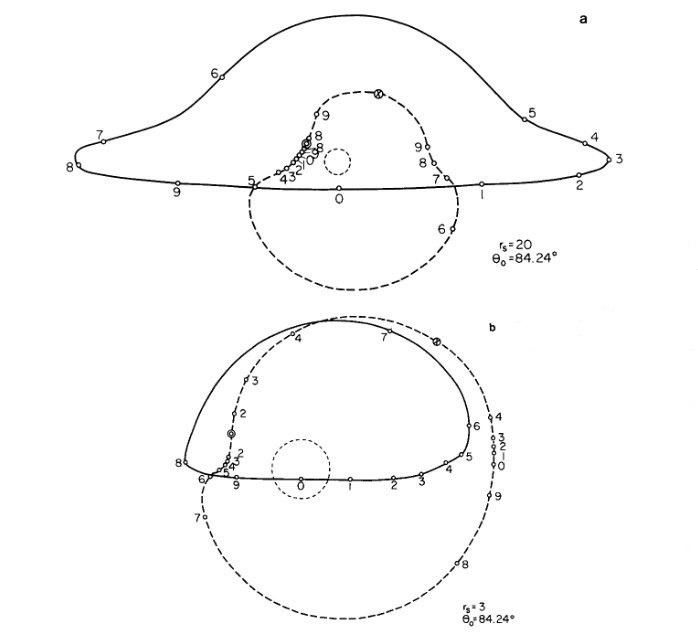
\includegraphics[width=0.4\linewidth]{img/Cunningham-Bardeen-1973-2images-2}
	\caption{The path(s) of a light source in the Kerr metric. \cite{cunningham1973optical}}
	\label{fig:Figure1.1}
\end{figure}

\vspace{1em}
	Cunningham released a paper in 1975 which presented the effects of redshift on an accretion disc in a Kerr black hole's equatorial plane\cite{cunningham1975effects}, but did not include an image of such effects.

\vspace{1em}
	In 1978, Jean-Pierre Luminet published the first image of an observer viewing the effects of gravitational lensing caused by a Kerr black hole\cite{luminet1979image}. This image was actually hand drawn using white ink, but the intensity of ink for each region was calculated using numerical techniques, taking into account the effect bolometric luminosity flux (change in brightness) of the accretion disc.

\begin{figure}[!ht]
	\centering
	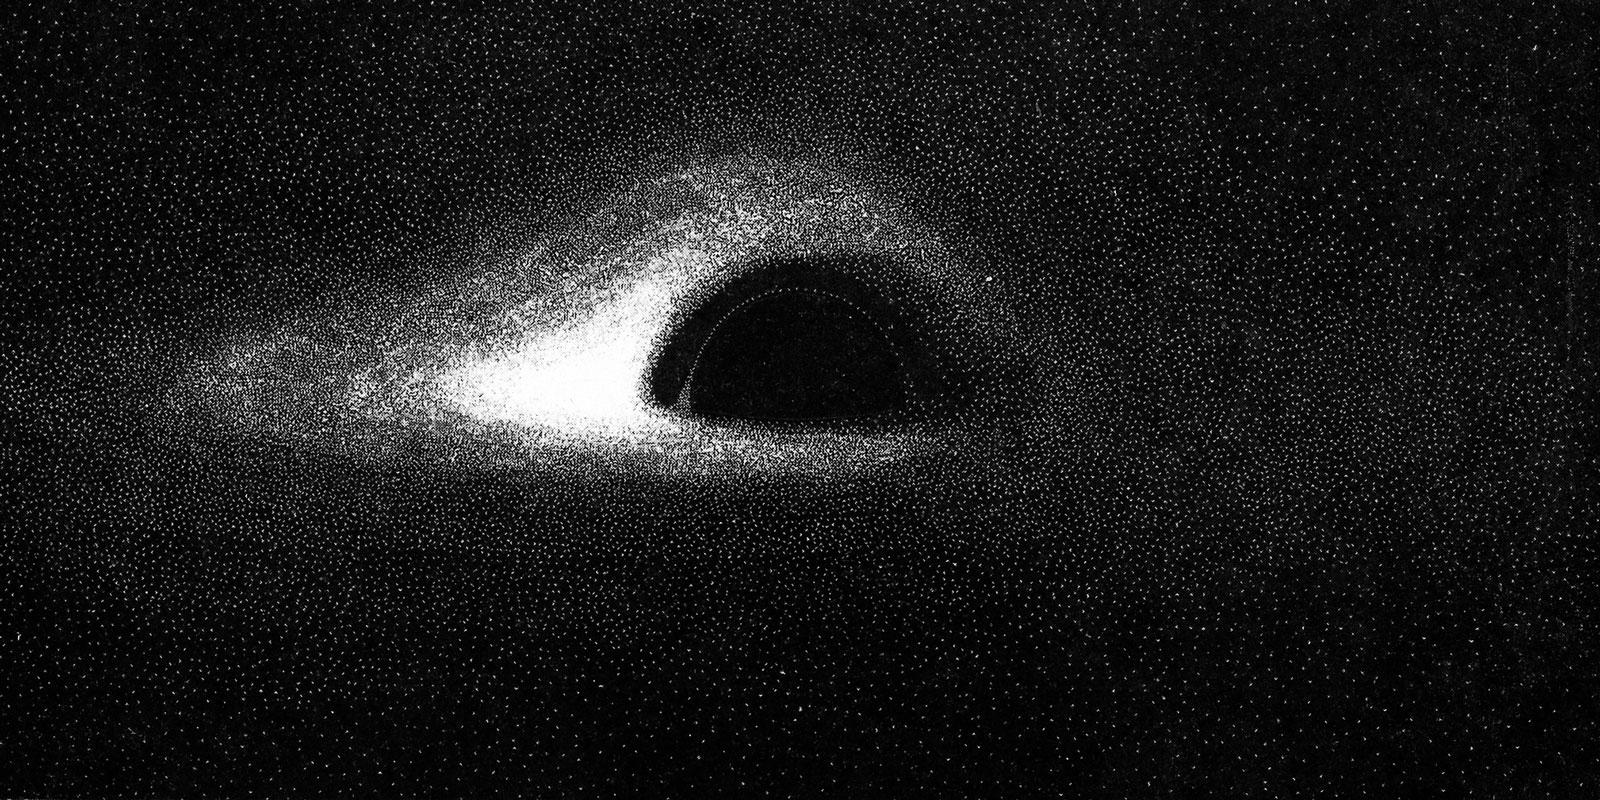
\includegraphics[width=0.45\linewidth]{img/Luminet-drawing}
	\caption{The first 'image' of a Kerr black hole. \cite{luminet1979image}}
	\label{fig:Figure1.2}
\end{figure}

\vspace{1em}
	In a paper by Fukue and Yokohama in 1988, the first non-bolometric coloured image of the same simulation as above was released\cite{fukue1988color}.

\section{1991-2022: Chasing realism}\label{sec:Section1.3}

	By 1990, the existence of black holes was all but confirmed, and the scientific community were in general agreement of their existence in the universe. This, coupled with more computational power, led to the field of black hole imaging becoming much more viable. In the era presented in this subchapter, far more than we could fit in has happened, but we present some of the key events.

\vspace{1em}
	Tragically given his untimely death at the age of 40, much of J.A. Mark's work is unpublished and unreleased, but what we do know is that in 1993 he produced the first animation of a flight inside a Schwarzschild black hole, and a flight over an elliptical orbit\cite{InfinitelyCurved}.

\vspace{1em}
	At this stage more and more realistic images could be generated, with the laws governing the magneto-hydrodynamics of black holes being proposed by Bardeen, Carter and Hawking in 1972\cite{bardeen1973four} and computers being capable of handling more complex computation.

\vspace{1em}
	In 2014, the release of the film Interstellar generated a surge of interest in realistic black hole modelling, as a focus was placed by director Christopher Nolan on realism in the film. Along with the release of the film came two papers\cite{thorne2015gravitational}\cite{thorne2015visualizing}, which pedagogically presented their process for generating realistic images and animations of Kerr black holes and Ellis-Thorne wormholes. The Kerr black hole shown in the film is unrealistic, even though it was generated mathematically; this is due to artistic choices made by director Christopher Nolan, leading to the lack of accounting for Doppler frequency shift and changes in energy flux.

\begin{figure}[!ht]
	\centering
	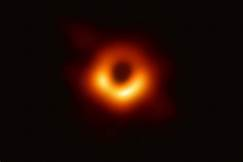
\includegraphics[width=0.45\linewidth]{img/M87}
	\caption{The well-known image taken of M87 in 2019. \cite{event2019first}}
	\label{fig:Figure1.3}
\end{figure}

\vspace{1em}
	Finally, the successful imaging of supermassive black hole M87 using the worldwide event horizon telescope\cite{event2019first} gave physical evidence as to the realism of previously generated images and, with that, evidence to further support the validity of Einstein's general theory of relativity. Who knows how far humans will progress in this field? Perhaps in the next 100 years we will have an image as high definition as the generated images presented throughout this paper of the black hole at the centre of the milky way - StrA*.

\vspace{1em}
	With an appreciation for the decades of work upon which we build our framework, we may now move onwards to introducing some more formal concepts which will allow our eventual generation of an image of a black hole.





\chapter{Introduction to general relativity}\label{chap:Chapter2}
	Albert Einstein’s theory of general relativity is a pivotal achievement in the scientific community, it is difficult to understate its importance to modern day theoretical astrophysics. In this chapter we will introduce some key concepts associated with general relativity to rely upon in later chapters.

\section{Special relativity}\label{sec:Section2.1}

	The idea of relativity predates Einstein quite substantially, the Galilean principle of relativity states the fundamental laws of physics are unchanged between frames of reference moving with constant velocity with respect to one another.

\vspace{1em}
	Einstein's special principle of relativity states\cite{einstein1923grundlage}: "If a system of coordinates K is chosen so that, in relation to it, physical laws hold good in their simplest form, the same laws hold good in relation to any other system of coordinates K' moving in uniform translation relatively to K."

\vspace{1em}
	The theory of special relativity is based upon the combination of this statement, and the postulate that the speed of light in a perfect vacuum is the same for any observer, independent of the light source and observer's motion.

\vspace{1em}
	Although Newtonian mechanics work remarkably well at low velocities, they break down as we approach the speed of light. It is in these scenarios in which we turn to relativity to accurately describe and analyse systems. Many ideas and effects using special relativity as a framework have been experimentally proven, such as the relativistic Doppler effect.

\vspace{1em}
	General relativity takes its name from the fact that it is a generalisation of special relativity and the Newtonian theory of gravity, covering systems in which gravitational fields are present. In this paper we will be using little from special relativity, but as it is contained within general relativity is it worth having an awareness of its basis.

\section{Geodesics}\label{sec:Section2.2}
	
	In 1915, in revelatory work analogous to that of Maxwell and Faraday on the unification of electromagnetism and the changing of perspective in electromagnetic fields which avoided action at a distance, Einstein formalised gravity not as a force, as it is thought of in Newtonian physics, but as the curvature of spacetime. Spacetime is the 4-dimensional field we exist in; one dimension representing time, and three space. 

\vspace{1em}
	The path, over time, of an object acted upon solely by gravity can be thought of as moving along curved spacetime, with the path being a straight line if the effects of gravity are non-existent. Such a path through curved spacetime is called a geodesic, and equations of motion in general relativity are governed by constants derived from geodesic equations – which in turn are derived from the curvature of regions of spacetime. A geodesic through spacetime which a test particle (or indeed a person) exists upon, is called it's worldline, for example all humans have their own worldline, which describes their movement through spacetime from birth to death.

\vspace{1em}
	This naming of a worldline can help us to define something like the event horizon of a black hole in a new way. One way of defining an event horizon is the surface around a singularity at which a test particle would have to travel at the speed of light in a vacuum to stay stationary. Our new definition would be that the conditions on the space and time coordinates change such that instead of time having to move forwards and space being free, the space coordinates for any worldline will end at the singularity. It is just a matter of how long this takes.

\vspace{1em}
	The origins of considering curved spacetime come from Riemannian geometry, which is a form of differential geometry; the study of curvature and surfaces. Using this relatively pure field, we can take many theorems, properties and relations with regard to curves and surfaces, and apply them to the curvature of spacetime.

\vspace{1em}
		We see in figure \ref{fig:Figure2.1} a common representation of the curvature of spacetime. This is actually an artist's rendition of an embedding diagram, since we are trying to visualise four dimensions as a plane, we must embed our higher dimensional image such that spacetime is represented as a flat plane. We can then visualise to what extent bodies of mass affect the curvature of this plane. Naturally if there is any curvature it ceases to be a plane, but it is called as such because this is its form under no gravitational effects.

\begin{figure}[!ht]
	\centering
	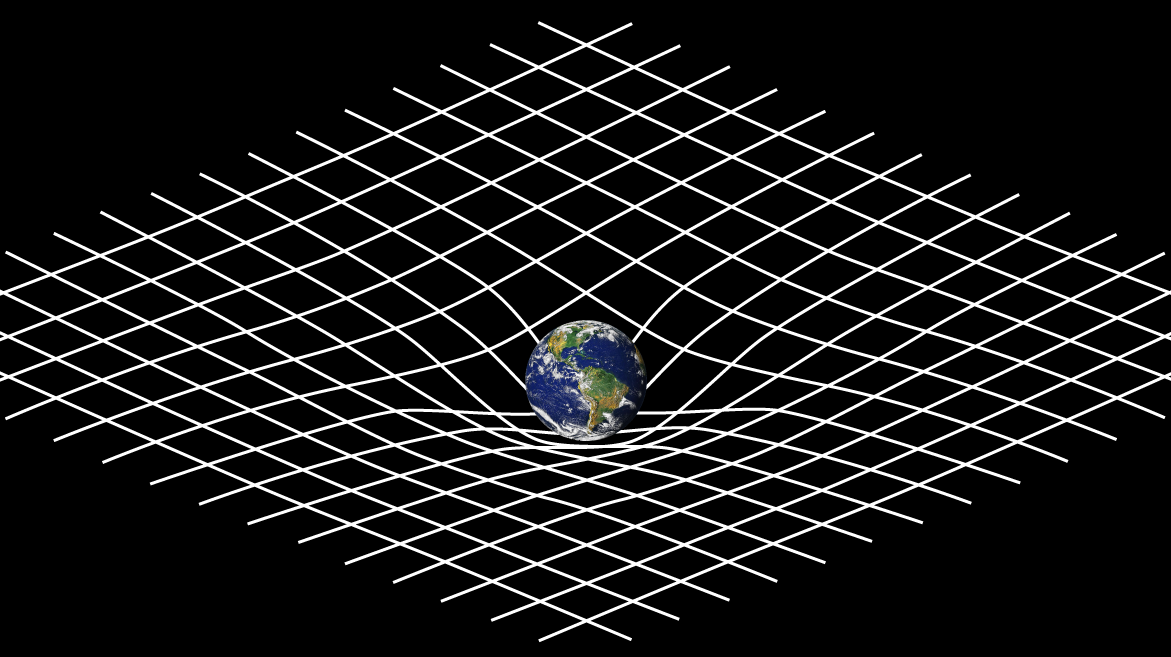
\includegraphics[width=0.5\linewidth]{img/curved-spacetime}
	\caption{An embedding diagram of curved spacetime.}
	\label{fig:Figure2.1}
\end{figure}

\vspace{1em}
	Above we mentioned the geodesic, and the way we introduced them was a simplification. The formal definition of a geodesic is a constant speed curve with zero geodesic curvature. They can be thought of as generalisations of straight lines in curved space. In general relativity geodesics fit into three categories:

\vspace{1em}
\begin{itemize}
  \item Time-like geodesics - A time-like geodesic describes the worldline of a test particle of non-zero mass $\Rightarrow$ travelling below the speed of light in a vacuum.
  \item Light-like geodesics - A light-like (or null) geodesic describes the worldline of a test particle of zero mass $\Rightarrow$ travelling at the speed of light in a vacuum.
  \item Space-like geodesics - Spacelike geodesics have little place in relativistic modelling as they do not represent the worldline of a particle of mass or photon.
\end{itemize}

\vspace{1em}
	One key thing to note is that a worldline cannot change from time-like/light-like to space-like, this will be of use in section \ref{sec:Section4.4}.

\vspace{1em}
	 In this paper, a null-geodesic will always be describing the worldline of a photon in a metric. Geodesic equations can be thought of as a generalisation of Newton's second law of motion, taking into account the curvature of the spacetime one chooses. That is, instead of F=0 $\Rightarrow$ a=0, we have that F=0 implies that acceleration is sufficient to keep the motion in a straight line in Euclidean space.

\section{Metrics and conventions}\label{sec:Section2.3}

\vspace{1em}
	Metrics are sections of spacetime which are solutions to Einstein’s field equations, the equations central to his general theory, relating matter distribution in an area of spacetime to its geometric properties. As an example, the simplest solution to these field equations describing a black hole is the Schwarzschild metric. A metric is generally given in line notation, which informs one how a small change in spacetime relates to changes in the variables we consider the object to be moving in.

\vspace{1em}
	Christoffel symbols are a useful notational timesaver, as they show up in many sections of Riemannian geometry, and so also general relativity. Tensors and scalars are crucial on a more academic level, and will be mentioned sparingly in the paper, but this by no means gives a sense as to how extensively they are studied when formulating and analysing metrics.

\vspace{1em}
	Christoffel symbols are related to the coefficients in the line metric, and consider all relations between variables. Below is the general form of the Christoffel symbol using Einstein's summation convention\cite[pg. 13-14]{albert1916foundation}:
	
	\[{\Gamma^\lambda}_{\mu\nu} = \frac{1}{2}g^{\lambda{l}}(\partial_{\nu}g_{\mu{l}} + \partial_{\mu}g_{l\nu} + \partial_{l}g_{\mu\nu}).\]
	
\vspace{1em}
	Here, g is the matrix of coefficients in the metric. The matrix g is also called the metric but this is as it determines the line notation completely. $g_{ij}$ is the (i,j)'th component of g, and $g^{ij}={g^{-1}}_{ij}$ is the (i,j)th component of the inverse of g.

\vspace{1em}
	Below is the general form of a geodesic equation\cite[pg. 156-157]{schutz2009first}:

	\[\frac{d^2 \gamma^\lambda}{dt^2} + {\Gamma^\lambda}_{\mu\nu} \frac{d\gamma^\mu}{dt} \frac{d\gamma^\nu}{dt} = 0.\]

\vspace{1em}
	As is common in papers studying light and the astronomical, we will be using natural units: that is, we will be taking c=G=1. This results in non-SI units, but conversion is possible and generally simple. A distance of 1 will correspond to $1$(s) $*$ c($ms^{-1}$) = the distance travelled by light in a vacuum in one second.

\vspace{1em}
	The celestial sphere from a point in space is an image of all the points taken to be arbitrarily far away. Using a distance we often take in this paper to be our celestial radius about Earth, it is the sky in all directions excluding the Moon, Mercury and Mars. Here the 'arbitrary distance' is t=1000, so the distance light travels in a vacuum in 1000 seconds.

\vspace{1em}
	Now that we have a knowledge of some of the foundations of relativity, we are ready to explore metrics describing black holes in the next chapter.






\chapter{Schwarzschild black holes}\label{chap:Chapter3}

	Equipped with the equations of motion derived from the geodesic equation determined by the metric we are using; we can find the path of light with certain initial conditions in such a metric by solving these equations numerically. In this chapter we will work towards generating an image of such a path.

\section{The Schwarzschild metric}\label{sec:Section3.1}

	Though black holes are remarkably complex, the no-hair conjecture states that they are defined entirely by only three externally observable parameters - mass, spin (angular momentum) and charge. This has actually only been partially proved, and counter examples exist in space higher than four dimensions, however it is generally accepted for astrophysical black holes.

	All black holes must have non-zero mass to be well defined, but the addition of charge and spin can change the properties significantly (for example, a black hole with zero spin has spherical symmetry). However, the inclusion of non-zero spin removes this symmetry, making equations of motion in the metric describing the black hole much more complex. Here is a table of the most commonly used metrics to describe each kind of black hole:

\vspace{1em}
\begin{center}
	\begin{tabular}{l l l}
		\toprule
		\textbf{ } & \textbf{Spin} & \textbf{No Spin}\\
		\midrule
		\textbf{Charge} & Kerr-Newman & Reissner-Nordström \\
		\midrule
		\textbf{No Charge} & Kerr & Schwarzschild \\
		\bottomrule
	\end{tabular}
	\captionof{table}{Metrics commonly to describe black holes}
\end{center}

\vspace{1em}
	Naturally, one could use the Kerr-Newman metric and simply take spin and/or charge to be zero and it would be equivalent to one of the other metrics, so objectively this is the most useful and general metric. However, if we know that we are uninterested in one of the variables it complicates things for us to abstract our work to allow for changing this variable.

\vspace{1em}
Later in this paper we will take a look at the Kerr metric, which can describe a rotating, non-charged black hole. But for now, we are interested in the Schwarzschild metric - given in line notation by: 

	\[{ds^{2} = {\left(1-\frac {2M}{r}\right)}^{-1}} {dr^2} + {r^2}({d\theta ^2} + {\sin ^2}{\theta}{d\phi ^2}) -{\left(1-\frac {2M}{r}\right)}{dt^2}.\]

\vspace{1em}
	Since the metric is spherically symmetric, we see that every path will always be contained in a plane intersecting the centre of the black hole (see figure \ref{fig:Figure3.2} (left)). Therefore, without loss of generality we can take ${\theta}=\frac{\pi}{2}$ and observe from 'above’ the equatorial plane to see the path of such a light ray in the plane.

\section{Coordinate systems}\label{sec:Section3.2}

	Looking ahead, we would like to model how a black hole affects a cameras view of a celestial sphere. To do this we must make two choices regarding coordinates and frames of references; firstly, we must choose which coordinates to use when forming the metric - this can be seen as the overarching coordinate system with its centre in the middle of the black hole, secondly a coordinate system must be chosen with regard to our camera.

\vspace{1em}
	For the Schwarzschild metric both choices are quite naturally spherical polar coordinates, we may also freely switch between Euclidean coordinates and spherical polar coordinates as they represent the same inertial system. The celestial sphere is centred at the observer, so is defined by our cameras coordinate system.

\vspace{1em}
	This choice is important to define to start as it affects how we give our metric, for example the Schwarzschild metric presented in section \ref{sec:Section3.1} is given with respect to spherical polar coordinates.

\section{Deriving the equations of motion}\label{sec:Section3.3}
	
	Using the Hamiltonian formalism, we may find the equations of motion governing a photon in the Schwarzschild metric, we aim to do this now:

	Observing the fact that the Schwarzschild metric is time independent implies that the energy of a photon in the metric will be constant. Similarly, independence from the variable $\phi$ leads us to see that the $\phi$-component of the angular momentum of a photon in the Schwarszchild metric remains constant. We call these constants E (=-$p_0$) and L (=$p_\phi$) respectively. Since we take ${\theta}$ to be constant, $p_\theta$=0 as the angular momentum in the $\theta$ plane is proportional to $\frac{d\theta}{dt}=0$.

\vspace{1em}
	For the other components of the photon's momentum:

	\[p^0 = g^{00}p_0 = \frac{rE}{r-2M},\]
	\[p^r = \dot{r},\]
	\[p^\phi = g^{\phi\phi}p_\phi = \dot{\phi} = \frac{L}{r^2}.\]

\vspace{1em}
	Using the equation $p \cdot p$=0 we see that:

	\[-\frac{rE^2}{r-2m}+\frac{r\dot{r}^2}{r-2M}+\frac{L^2}{r^2}=0.\]

\vspace{1em}
	This equation can be solved, leading to the equation:

	\[\dot{r}^2 = E^2-\frac{L^2(r-2M)}{r^3} = E^2 + V^2.\]

\vspace{1em}
	Here we let V=V(r) for ease of notation.

\vspace{1em}
	Then, taking the time derivative of both sides of this equation:

	\[2\dot{r}\ddot{r} = -\frac{d}{dr}(V^2)\dot{r}.\]

\vspace{1em}
	Calculating $\frac{d}{dr}(V^2)$ shows that the equations of motion of a photon in the Schwarzschild metric are governed by:

	\[\ddot{r} = -\frac{1}{2}\frac{d}{dr}(V^2) = -\frac{L^2(3M-r)}{r^4},\]
	\[\dot{\phi}=\frac{L}{r^2}.\]

\vspace{1em}
	Where M is the mass of the black hole, r is the radial distance from the centre of the black hole, and $\phi$ is the angle from the positive x axis to the light ray.

\vspace{1em}
	In this section, usually instead of the time variable t, a variable $\lambda$ related to t is used, but as we are not interested in modelling realistic animations, taking t as our variable does not affect the end result. The derivations in this subchapter were based on \cite[pg. 283-285]{schutz2009first}.

\section{Modelling a photon path}\label{sec:Section3.4}

	The simplest method of numerically solving the equations derived in section \ref{sec:Section3.3} is to split the equations into a system of coupled first order differential equations. Then, use a numerical approximation to update r, $\dot{r}$ and $\phi$ for each point in a time array. If we keep track of r and $\phi$ for all points in the time array we can then plot the path.

\vspace{1em}
	This method is both the simplest and most effective for solving second order ODE’s numerically, the only difference between a ‘bad’ and ‘good’ method would be the choice of numerical approximation method to solve the first order ODE’s.

\vspace{1em}
	One thing to be careful about is that there is a coordinate singularity at r=2M, meaning this surface is ill-described by our metric, so we cannot have an initial position in this region, and ideally while keeping track of r, cut the process off when r=2M (if not during the process to save computation, we cut the photon off after the process). This is actually the event horizon of the Schwarzschild black hole, and for a long time was considered a singularity associated with the metric, we will not prove the contrary here but a proof of the same for the Kerr metric is given in section \ref{subsec:Subsection4.3.3}.

\vspace{1em}
	Below are the coupled differential equations equivalent to the equations of motion:

	\[\dot{r}= s,\]
	\[\dot{s}=-\frac{L^2(3M-r)}{r^4},\]
	\[\dot{\phi}=\frac{L}{r^2}.\]

\vspace{1em}
	For a plot of the path of a photon (See figure \ref{fig:Figure3.1}), a suitable method in python is SciPy's solve\_ivp\cite{2020SciPy-NMeth}, using LSODA\cite{hindmarsh2005lsoda}. This is because the explicit Runge-Kutta method of order 5 (RK45)\cite{fehlberg1969low}, the inherent method used by solve\_ivp, is very efficient but not smooth, so finds the final position quickly and accurately but in few steps, meaning plots of paths look unrealistic. Later, when a plot is not required, we will be using RK45.

\vspace{1em}
	Using solve\_ivp allows one to keep track of an ‘event’, and return if the event took place. Moreover, one may choose to cut off the calculation process when such an event takes place. Naturally this is very useful in our case, since if we set an event at r=2M, we can prevent unnecessary computation beyond the event horizon (and of course have a simple method for finding out if a photon path enters the event horizon).

\begin{figure}[!ht]
	\centering
	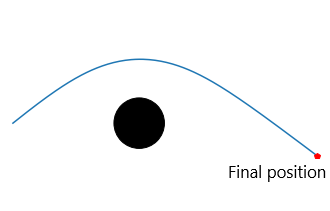
\includegraphics[width=0.4\linewidth]{img/Schwarzschildpath}
	\caption{The path of a photon in the equatorial plane of a Schwarzschild black hole.}
	\label{fig:Figure3.1}
\end{figure}

\subsection{Runge-Kutta-4 method}\label{subsec:Subsection3.4.1}

	The Runge-Kutta-4 method is a numerical approximation which solves a system of the form

\vspace{1em}
\[\dot{\mbox{X}}(\lambda) = \mbox{F}(\lambda,\mbox{x}(\lambda)).\]

\vspace{1em}
	Using the fact that a solution to such an equation satisfies:

\vspace{1em}
	\[\mbox{X}(\lambda+\mbox{h}) = \mbox{X} + \frac{\mbox{h}}{6}f_1(\lambda,\mbox{X}(\lambda))+f_2(\lambda,\mbox{X}(\lambda))+f_3(\lambda,\mbox{X}(\lambda))+f_4(\lambda,\mbox{X}(\lambda))+O(\mbox{h}^6),\]
	\[f_1(\lambda,\mbox{X}(\lambda)) = F(\lambda,\mbox{X}(\lambda)),\]
	\[f_2(\lambda,\mbox{X}(\lambda)) = F\left(\lambda+\frac{\mbox{h}}{2},\mbox{X}+\frac{\mbox{h}f_1(\lambda,\mbox{X}(\lambda))}{2}\right),\]
	\[f_3(\lambda,\mbox{X}(\lambda)) = F\left(\lambda+\frac{\mbox{h}}{2},\mbox{X}+\frac{\mbox{h}f_2(\lambda,\mbox{X}(\lambda))}{2}\right),\]
	\[f_4(\lambda,\mbox{X}(\lambda)) = F\left(\lambda+\mbox{h},\mbox{X}+\mbox{h}f_1(\lambda,\mbox{X}(\lambda))\right).\]

\vspace{1em}
	Here h is our step-size, which can be varied depending on how quickly the system is changing at a given time. Since we take up to order 5, this is the equations RK45 are based upon. The proof of this relation involves taking the Taylor expansion of X.

\section{Generating an image of the effects of gravitational lensing}\label{sec:Section3.5}

	We now have the means to start thinking about how to model a black hole, with any given celestial sphere and initial conditions.

\subsection{Outline of the method}\label{subsec:Subsection3.5.1}

	Firstly, we would like to find an equation linking launch angle and L, as this would allow us to choose a launch angle and calculate the required initial conditions for such an angle.

\vspace{1em}
	Then, to model a Schwarzschild black hole we will first find the minimum angle one may fire a photon from the camera without the photon being absorbed by the singularity. For all angles between this minimum angle and $\frac{\pi}{2}$, we will find a relation between angle fired and final angle after a sufficient amount of time.

\vspace{1em}
	We will then conceptualise a pinhole camera, with its focal point, distance r from the centre of the black hole, the position of our camera which fires light rays. Using the relation outlined above, we can take any given straight line of pixels which passes through the centre of the image we take as our celestial sphere. This line represents a plane in which photons may travel in. Then by rotating the plane we are working in to become the equatorial plane (see figure \ref{fig:Figure3.2} (right)), or equivalently rotating the line of pixels to lie on the x axis, and performing a calculation before rotating back to our original plane; we may find where each pixel ends up on the celestial sphere.

\begin{figure}[!ht]
	\centering
	\begin{minipage}{0.5\textwidth}
		\centering
		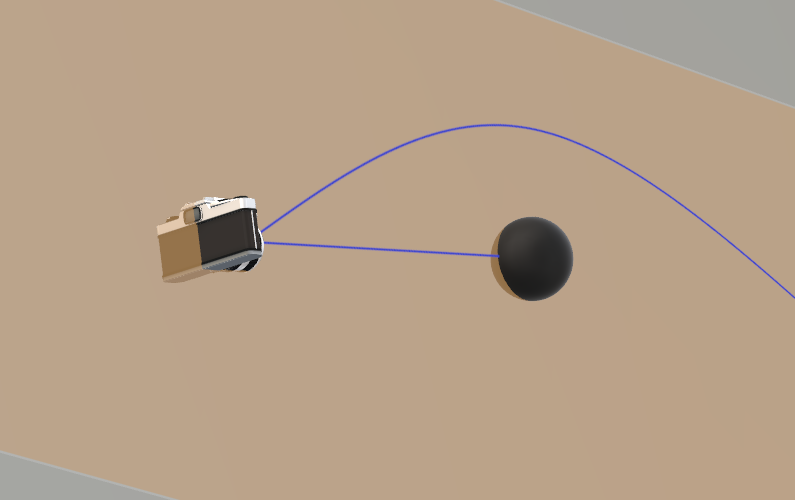
\includegraphics[width=0.8\linewidth]{img/plane}
	\end{minipage}%
	\hfill
	\begin{minipage}{0.5\textwidth}
		\centering
		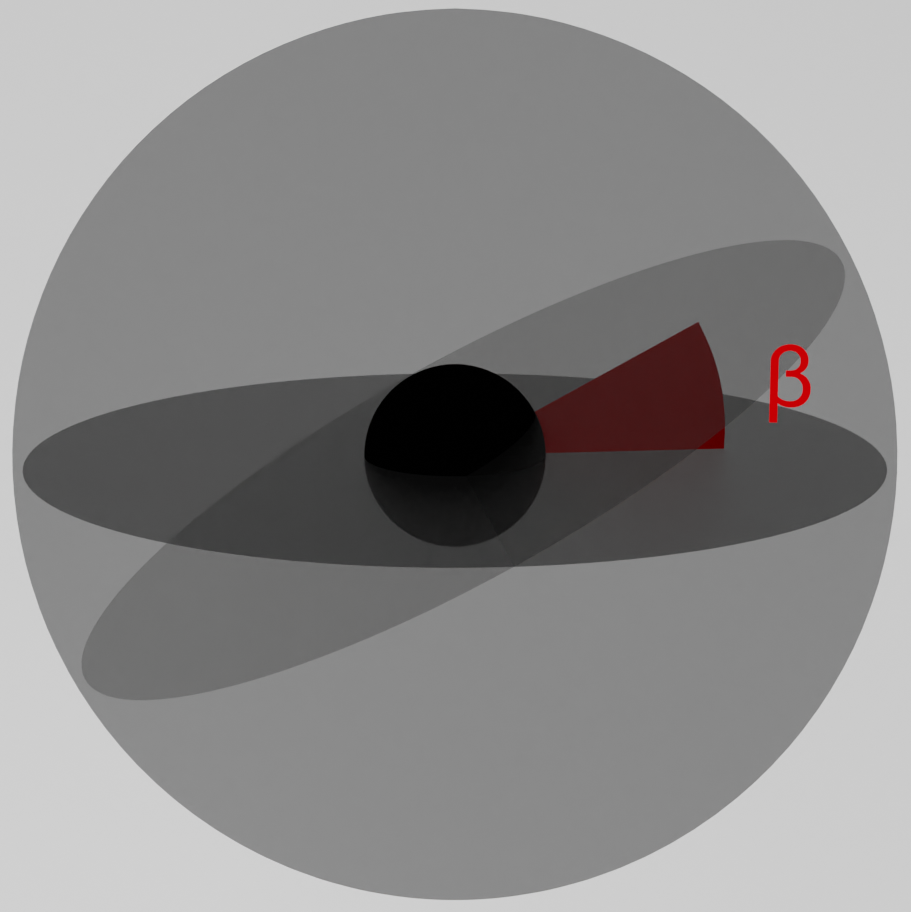
\includegraphics[width=0.72\linewidth]{img/inclinationfigure}
	\end{minipage}
	\caption{A model demonstrating the plane formed by a photon path and the line connecting initial position to the centre of the black hole (left). A model showing the inclination angle required to transform the equatorial plane to a general plane passing through our initial position and the centre of the black hole (right).}
	\label{fig:Figure3.2}
\end{figure}

\subsection{How to acquire the launch angle}\label{subsec:Subsection3.5.2}

	For the rest of this paper, we refer to a given photon's launch angle by $\alpha$. We would like to use the equations of motion at t=0 to discover what value of L is needed with given $\dot{r}$(0) to obtain a desired value of $\alpha$.

\vspace{1em}
	As we are in polar coordinates, 

	\[(x, y) = (r\cos(\phi), r\sin(\phi)) \Rightarrow (\dot{x}, \dot{y}) = (\dot{r}\cos(\phi) - r\dot{\phi}\sin(\phi), \dot{r}\sin(\phi) + r\dot{\phi}\cos(\phi)).\]
	
\vspace{1em}
	Via basic geometry in our plane of motion, we see that:
			
	\[\tan(\alpha) = \frac{\dot{y}(0)}{\dot{x}(0)} = \frac{\dot{r}(0)\sin(\phi(0)) + r(0)\dot{\phi}(0)\cos(\phi(0)}{\dot{r}(0)\mbox{cos}(\phi(0)) - r(0)\dot{\phi}(0)\sin(\phi(0))}.\]

\vspace{1em}
	So, we obtain:

	\[ L = \frac{r(0)\dot{r}(0)(\cos(\phi(0))\tan(\alpha)-\sin(\phi(0))}{\cos(\phi(0))+\sin(\phi(0))\tan(\alpha)}.\]
	
\vspace{1em}
	To find the minimum angle at which a light ray escapes the gravitational pull of the black hole, we send out a number of photons with increasing launch angle from 0 to $\frac{\pi}{2}$, then, as soon as an angle does not lead to the crossing of the event horizon, we repeat this process with much greater precision between the previous (terminated) and current (not terminated) angle. This leads to an accurate $\alpha_{min}$.

\subsection{The relationship between launch angle and final angle}\label{subsec:Subsection3.5.3}

	By solving the equations of motion using launch angles from $\alpha_{min}$ to $\frac{\pi}{2}$, and plotting $\alpha$ on the x-axis and $\alpha^{'}$ on the y axis; where  $\alpha^{'}$ is the angle from the camera to the final position of the light ray (See figure \ref{fig:Figure3.2} (left)), we may find the relationship between $\alpha$ and $\alpha^{'}$. For $\alpha$ between -$\frac{\pi}{2}$ and -$\alpha_{min}$ we may take -f(-$\alpha$), where f is the function relating the two. Here we have covered -$\frac{\pi}{2}$ to $\frac{\pi}{2}$ radii, more than a full field of view.

\vspace{1em}
	When $\alpha \approx \alpha_{min}$ or $-\alpha \approx -\alpha_{min}$ the light ray might semi-orbit or even fully orbit the black hole, meaning we must be careful in our method of calculating $\alpha^{'}$. To avoid a discontinuous plot of the function (see figure \ref{fig:Figure3.3} (right)), we keep track of the change in $\phi$, the angle from the centre of the black hole to the current position of the photon. When taking this value modulo $2\pi$, we can see how many orbits the ray has undergone. When modelling a photon path there is no difference in which angle we take, modulo $2\pi$.

\begin{figure}[!ht]
	\centering
	\begin{minipage}{0.5\textwidth}
		\centering
		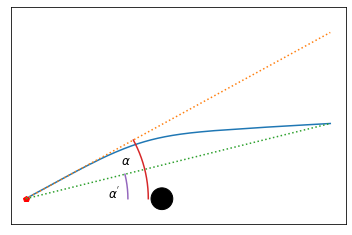
\includegraphics[height=0.5\linewidth]{img/alpha_alpha-prime}
	\end{minipage}%
	\hfill
	\begin{minipage}{0.5\textwidth}
		\centering
		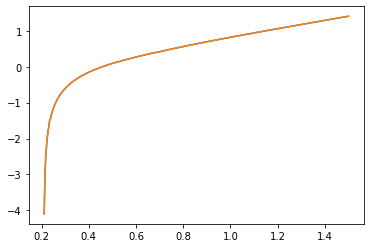
\includegraphics[height=0.5\linewidth]{img/alpha-prime_f(alpha)}
	\end{minipage}
	\caption{A figure showing initial and final angle: $\alpha$ and $\alpha^{'}$ respectively (left). A plot of the function relating the two (right).}
	\label{fig:Figure3.3}
\end{figure}

\subsection{Modelling the black hole}\label{subsec:Subsection3.5.4}
	
	As outlined in section \ref{sec:Section3.1}, here we will give our code a star field to treat as a celestial sphere, and see how a black hole affects the image. To do this, the first thing we calculate is the distance in pixels from the centre of the picture to a corner, this will correlate directly to $\frac{\pi}{2}$ radians. Then, for every pixel (i,j) on the original image we 'rotate' the plane we are working in to treat it as the equatorial plane of the black hole; we can do this due to the symmetries implied by the Schwarzschild metric. 

\vspace{1em}
	After calculating the angle $\alpha$ implied by the distance from the pixel (i,j) to the centre of the image (0,0), we use numerical interpolation on our relationship between $\alpha$ and $\alpha^{'}$ to calculate the angle along the plane at which the light ray would end. Then by converting this angle back to distance, and performing an inverse rotation to arrive back in our original plane, we update a copy of the picture by switching the current pixel with the closest pixel to the end point on the original picture.

\subsection{The importance of a proper celestial sphere}\label{subsec:Subsection3.5.5}

	One issue that we run into when not using an image covering $4\pi$ steradians (2 dimensional equivalent of radians, $4\pi$ covering a full sphere), is that any ray which leaves the area covered by the original image leads to a black pixel. This leads to an irregularly shaped black hole (See figure \ref{fig:Figure4.3}), if the image we use as a celestial sphere is circular, the black hole would seemingly look ordinary, as the irregularities would be smoothed out horizontally and vertically, but would be too large due to the photon paths cut off which simply leave the original field of view. 

\vspace{1em}
	Our solution to this will be to use a HDRI image, which indeed covers $4\pi$ steradians, we will be keeping models in this form, this is commonly done; as it is simple to convert a HDRI image back to an ordinary POV image, but we are then limited to a small section of the information which can be seen in the original HDRI image. For example, if one wanted to create a virtual reality image of a camera, one could rely solely upon one of these HDRI images.

\vspace{1em}
	This does however change our previous method slightly, as HDRI images are designed to have the coordinates directly correlated to $\theta$ and $\phi$ in 3-d polar coordinates centred at the cameras position, covering $\pi$ and $2\pi$ respectively (leading to a full field of all possible views from the point), so instead of the distance to the corner of our image, we take half the height of our image to find the factor, as this would correlate to $\frac{\pi}{2}$ radians. We are then limited to a maximum angle of $\frac{\pi}{2}$ radians, meaning we may update the image only in a circle centred at the middle of the image, with radius $\frac{\mbox{height}}{2}$. Figure \ref{fig:Figure3.5} is a cropped image of inside this circle.

\vspace{1em}
	To be able to model light rays with launch angles above $\frac{\pi}{2}$, and hence to be able to generate a full HDRI image, one must switch to the more general method of modelling black holes, relativistic ray tracing, in which we solve the equations of motion numerically for each pixel without using the relationship between $\alpha$ and $\alpha^'$. As the purpose of this section is to explore and explain efficient solutions we will not cover modelling a Schwarzschild black hole via relativistic ray tracing, however, in chapter \ref{chap:Chapter4} we will be using this method to model light in the Kerr metric.

\begin{figure}[!ht]
	\centering
	\includegraphics[width=0.8\linewidth]{img/8kstarfield-special}
	\caption{A model highlighting areas affected by the limited size of the background image.}
	\label{fig:Figure3.4}
\end{figure}

\section{Analysing the image}\label{sec:Section3.6}

	Now that we have a high-quality model for the effects of gravitational lensing caused by the Schwarzschild metric on a celestial sphere, we can take a look at the image and note some key features.

\begin{figure}[!ht]
	\centering
	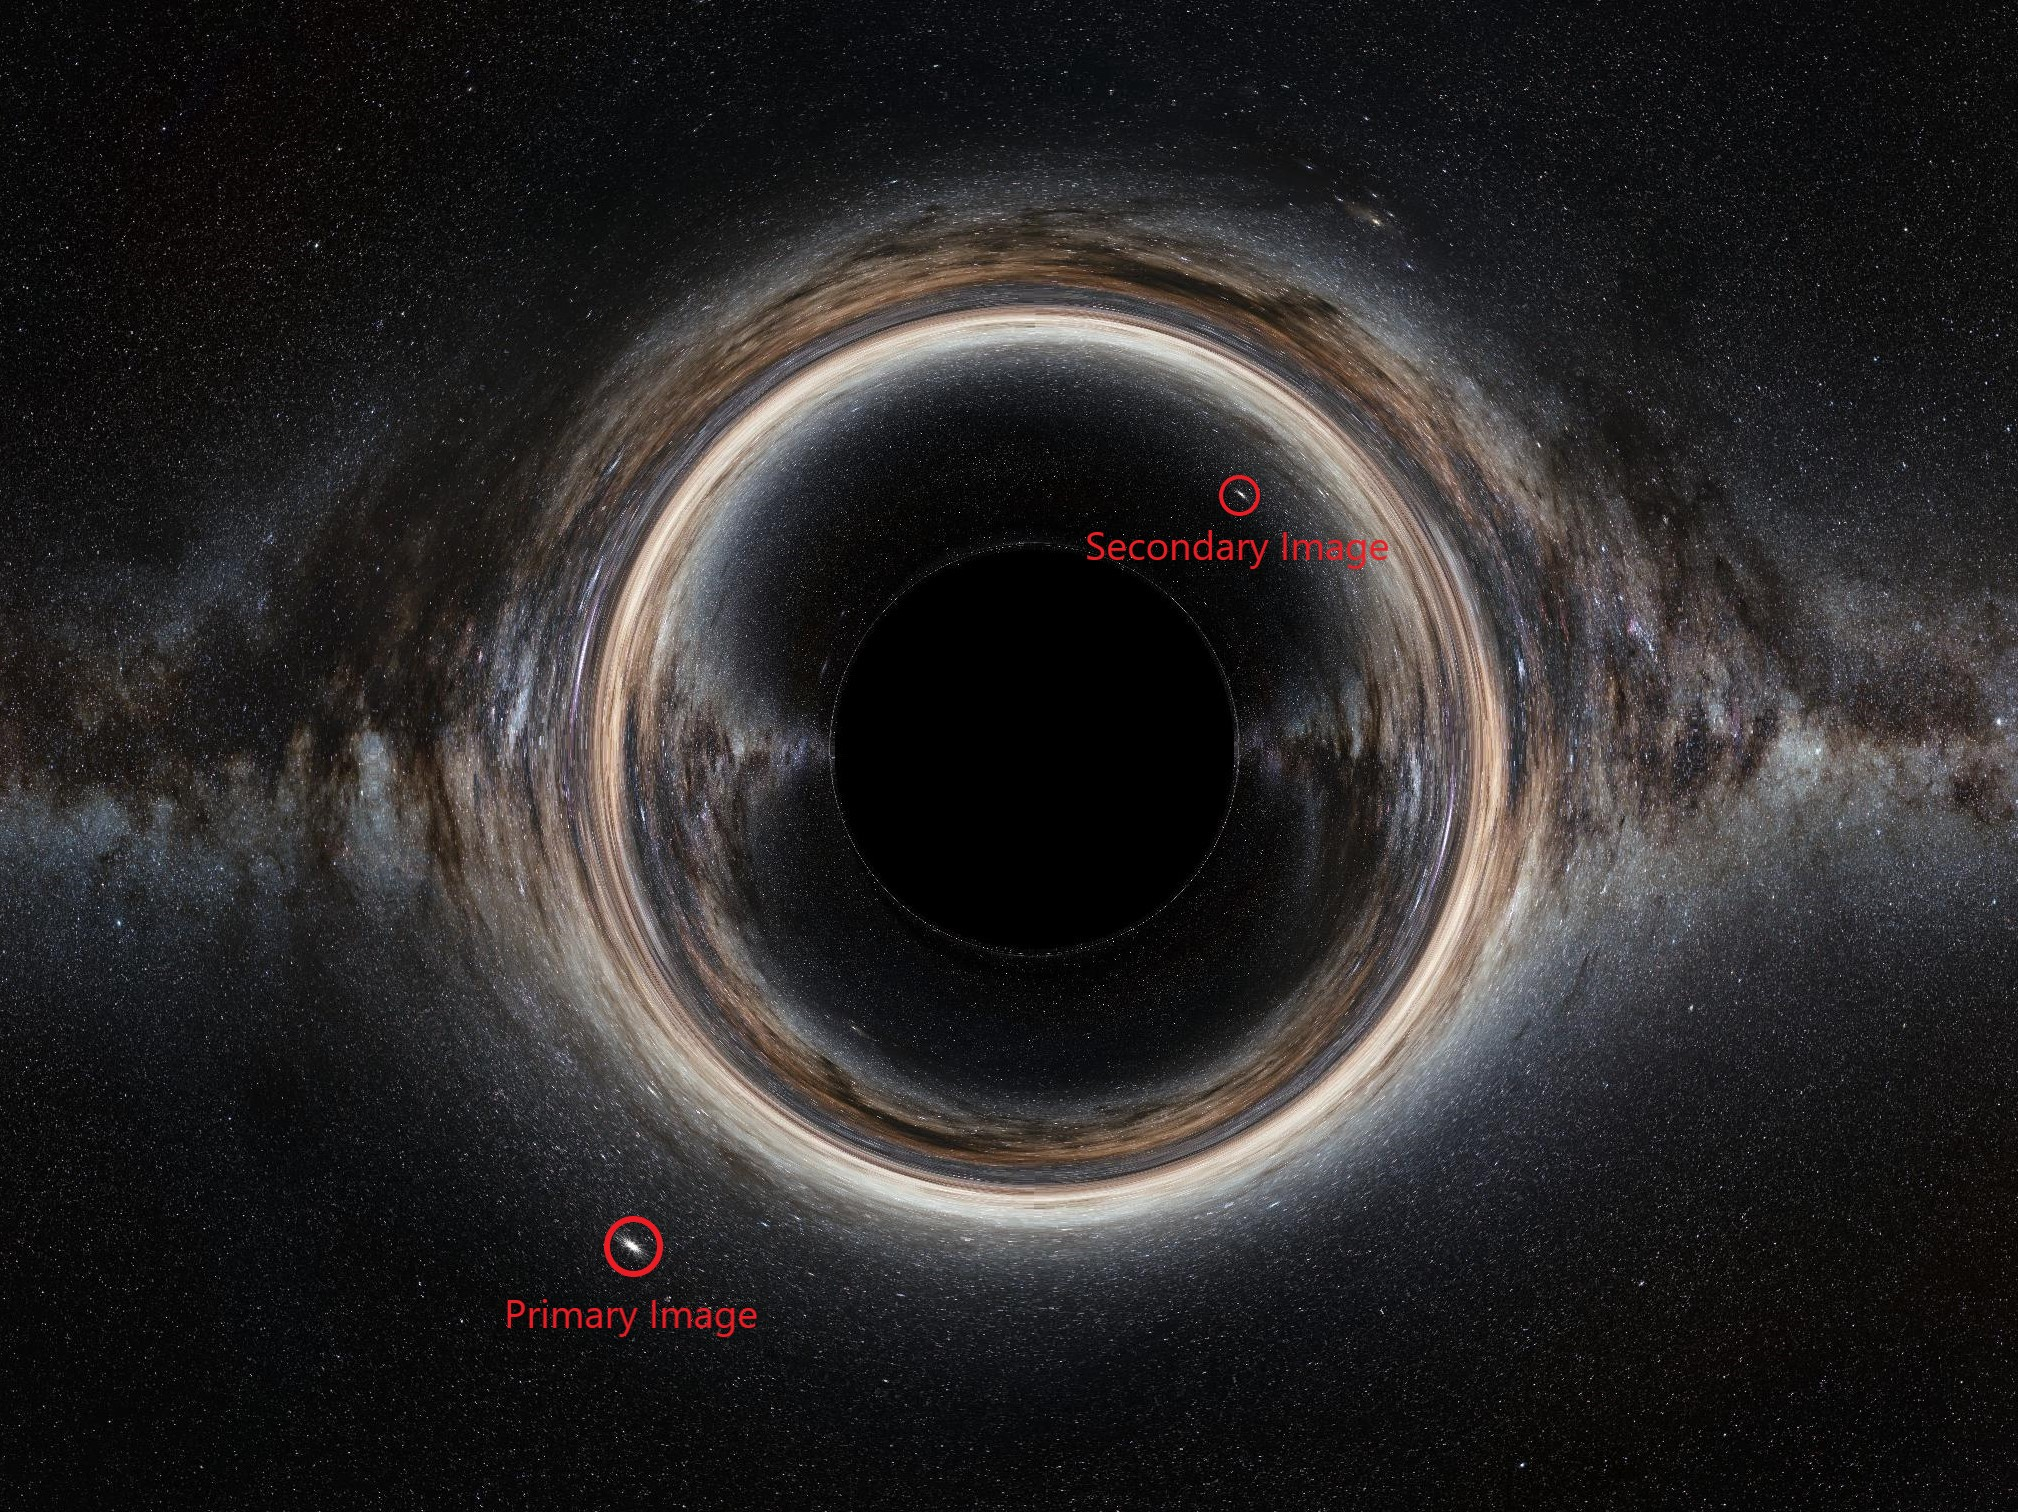
\includegraphics[width=0.8\linewidth]{img/milkyway-SC}
	\caption{A model of a Schwarzschild black hole using a HDRI image, cropped.}
	\label{fig:Figure3.5}
\end{figure}

	First, we note the purpose of using a HDRI image in the highlighted region of figure \ref{fig:Figure3.4}, and see the circular nature of the shadow caused by the event horizon in figure \ref{fig:Figure3.5}, this stands to reason and is what we expect to see. 

\vspace{1em}
	The shadow can often be called the event horizon, but this is a misleading name, as it is really a shadow caused by photons being absorbed by the event horizon. This is a subtle distinction but the front side of the event horizon only takes up about half the area of the shadow, the rest is caused by photon paths which hit the back of the event horizon - or even orbit the black hole a number of times and then hit the horizon. Naturally we can fine-tune the angle we fire a photon at and make a photon orbit the black hole an arbitrary number of times - so the shadow is actually an image of an infinite number of copies of the whole surface of the event horizon.

\vspace{1em}
	The above description would be correct if the image was perfectly high definition, but due to image size there is a maximal number of orbits we can make a photon orbit, namely caused by the final layer of black pixels forming the shadow.

\vspace{1em}
	As seen in figure \ref{fig:Figure3.5}, we see that there are multiple images of notable features, including the star circled. This is due to the multiple path's photons may take to reach a point in space in the Schwarzschild metric. Unlike in the spacetime we are used to and experience, where photons travel in near straight-lines; photon paths are 'bent' sufficiently in a black hole's gravitational field, that a photon may travel above and around a black hole to reach a point in space which may be reached by being bent slightly travelling below the black hole to begin with. This is specifically the case for the circled image; the primary image, caused by a photon travelling as directly as it can to the light source, is named as such since it is brighter and larger. The secondary image however requires a more convoluted path, above and around the black hole, so fewer photon paths reach the light source via this route, leading to a smaller and less bright image.

\vspace{1em}
	This phenomenon may be seen for every light source on the original HDRI image acting as our celestial sphere and, not only that; if we had a high enough definition image, we would see tertiary images and so on infinitely as we zoom in on the outer layer of the shadow. These images would become smaller and less intense as we move closer due to the fact that we are requiring photons to orbit the black hole more times each image further we look.

\vspace{1em}
	We see that in a circle around the centre of the shadow, an image is formed from one light source, this is because whichever light source lies directly behind the black hole in line with the camera has a circular primary image. Another way of thinking about this is that the shortest path to the point on the celestial sphere directly behind the black hole is to be bent back down to this point by the black hole, and since we have spherical symmetry, this angle is the same for whichever inclination we choose, as an interesting aside, this angle happens to be the y-axis intersection of the relation graph between $\alpha$ and $\alpha^{'}$. The circular image caused by this light source is named the Einstein ring of the black hole, and is very notable in figure \ref{fig:Figure3.5} due to the celestial sphere chosen.




\chapter{Kerr black holes}\label{chap:Chapter4}

	In this section we move on to more general black holes, specifically with non-zero spin. We will introduce the Kerr metric and analyse some of its key regions, and then examine the equations of motion of light in the Kerr metric. We take a more general backwards ray tracing approach to modelling light around a Kerr black hole, since the metric lacks spherical symmetry (meaning we cannot generalise to two dimensions), the interpolation method is significantly less efficient. As mentioned in section \ref{subsec:Subsection3.5.4} this method, although slower, has its upsides - notably freedom of initial launch conditions.
	
\vspace{1em}
	Therefore, we view our background image as a full 4$\pi$ steradian field of view, and for each pixel on the image, we calculate the required launch angle and inclination angle for a photon to reach this light source in ordinary spacetime. We then use these angles as initial conditions to see where the modelled photon ends up in the Kerr metric. Now, with a final position we can calculate the related angles to reach this position in ordinary spacetime and hence the related pixel on a HDRI image.

\section{The Kerr metric}\label{sec:Section4.1}

	The Kerr metric is used to describe a non-charged, rotating mass; often a black hole, with spin parameter per unit mass J=$\frac{a}{M}$, where M is the mass of the black hole and a is the spin parameter. J can range from -1 to 1 (an extreme Kerr black hole), with J=0 describing a Schwarzschild black hole.

\vspace{1em}
	When the absolute value of J is taken to be greater than one, the Kerr metric can be used to describe a naked singularity, which is a singularity with no event horizon surrounding it. The weak cosmic censorship hypothesis, proposed by Roger Penrose in 1969\cite{penrose1969gravitational}, suggests that no naked singularities exist in our universe. Since outside of singularities general relativity is deterministic (i.e., any systems evolution is perfectly predictable given initial conditions), this hypothesis leads to the conclusion that general relativity itself is a deterministic framework. This hypothesis has not been proved nor disproved and continues to be an area of interest in the scientific community, first and foremost among the aims being an appropriate formal presentation of the hypothesis.

\vspace{1em}
	The Kerr metric of a mass M, rotating with angular momentum a, can be given in line element in Boyer-Lindquist coordinates by \cite{boyer1967maximal}:

	\[-ds^2=d\tau^{2} = \left(1-\frac{2r}{\Sigma}\right)dt^2+\frac{4ar\sin^2(\theta)}{\Sigma}dtd\phi-\frac{\Sigma}{\Delta}dr^2-{\Sigma}d\theta^2-\frac{\chi\sin^2(\theta)}{\Sigma}d\phi^2.\]

\vspace{1em}
	With:
	
	\[\Delta(r) := r^2 - 2r + a^2,\]
	\[\Sigma(r, \theta) := r^2 + a^2\cos(\theta)^2.\]
	\[\chi = (r^2+a^2)^2-a^2\sin^2(\theta)\Delta.\]

\section{Coordinate systems}\label{sec:Section4.2}

	There are two commonly used coordinate systems to formulate the Kerr metric; Boyer-Lindquist coordinates\cite{boyer1967maximal}, and Kerr-Schild coordinates\cite{debney1969solutions}. In section \ref{sec:Section4.1}, we used Boyer-Lindquist coordinates, which are a form of 'stretched' spherical polar coordinates related to Euclidean spacetime by:

	\[t=t,\]
	\[x = \sqrt{r^2+a^2}\sin(\theta)\cos(\phi),\]
	\[y = \sqrt{r^2+a^2}\sin(\theta)\sin(\phi),\]
	\[z = r\cos(\theta).\]

\vspace{1em}
	Take note that as is the case in many coordinate systems, there are areas which are ill-defined in Boyer-Lindquist coordinates - namely for the equations of motion presented in section \ref{sec:Section4.5} when $\theta = 0\mbox{ or }\pi$, which corresponds to the z axis in three dimensional Euclidean space. A solution to this is to shift to a rotated Boyer-Lindquist system for any photon path which passes through ill-defined points. By 'stitching' these two coordinate systems together we may avoid any problems. A quicker fix is be to discount any photon paths which pass through this line as there are very few of them of a high-resolution image.

\vspace{1em}
	Although less commonly used, the Kerr metric was proposed in 1965; two years after Kerr first formulated it, in Kerr-Schild coordinates. These are coordinates used to describe linear perturbations to spacetime metrics, and are a set of Cartesian coordinates, in the case of the Kerr metric given by:

	\[g_{\alpha\beta} = \eta_{\alpha\beta} + 2H\kappa_{\alpha}\kappa_{\beta},\]
	\[\textbf{k} = (\kappa_x,\kappa_y,\kappa_z) = \left(\frac{rx+ay}{r^2+a^2},\frac{ry-ax}{r^2+a^2},\frac{z}{r}\right),\]
	\[H = \frac{r^{3}}{r^{4}+a^{2}z^{2}}\]
	\[k_0 = 1.\]

\vspace{1em}
	Here $\eta$ is the Minkowski tensor, describing flat Minkowski spacetime, and $\textbf{k}$ is a unit vector which we are using to perturb the Minkowski metric. Also, here r is not the usual radial component, but is defined through satisfying the equation:

\vspace{1em}
	\[\frac{x^2+r^2}{a^2+r^2}+\frac{z^2}{r^2} = 1\]

\vspace{1em}
	Generally, Boyer-Lindquist coordinates are a more helpful coordinate system to work in, especially when looking at photon paths, but Kerr-Schild has its advantages, notably when analysing the metric and its regions, often papers will use Kerr-Schild coordinates to analyse singularities, we will do just this and more formally introduce Kerr-Schild coordinates in section \ref{subsec:Subsection4.3.3}.

\vspace{1em}
	Another coordinate system which is growing more popular in recent years is Doran coordinates\cite{doran2000new}. Designed such that as one tends angular momentum towards 0, Doran coordinates collapse to Painlev\'e–Gullstrand coordinates\cite{painleve1921mecanique} describing the Schwarzschild metric. The Kerr metric is given in line element using Doran coordinates as:

	\[ds^2=-dt^2+(r^2+a^2\cos^2(\theta))d\theta^2+(r^2+a^2)\sin^2(\theta)d\phi^2+\]
	\[\left(\frac{r^2+a^2\cos^2(\theta)}{r^2+a^2}\right)\left\{dr+\frac{\sqrt{2Mr(r^2+a^2)}}{r^2+a^2\cos^2(\theta)}(dr-a\sin^2(\theta)d\phi)\right\}^2.\]

\vspace{1em}
	Some useful features include the fact that as we tend M to 0, the metric becomes the flat Minkowski metric in oblate spheroidal coordinates. Also, recalling notation for the inverse of the metric matrix, $g^{tt}=-1$ everywhere in Doran coordinates. The time coordinate in this metric acts in many ways as Newtonian time, representing the proper local time for a free-falling observer on some simple trajectories. 

\vspace{1em}
	Doran stated "Many physical phenomena are particularly clear when related to this time coordinate. The chosen coordinates also ensure that the solution is well behaved at the horizon."\cite{doran2000new} The metric is suited for numerical methods and study near the horizon is often best performed using Doran coordinates.

\subsection{Reference frame coordinates}\label{subsec:Subsection4.2.1}

	As we previously did for the Schwarzschild case in section \ref{sec:Section3.2}, as well as defining which coordinates we are using for the metric, we will now also define which coordinate system we use for our camera, and consequentially fix its frame of reference. 

\vspace{1em}
	We will be modelling the camera as a fiducial, i.e. locally non-rotating, observer. Crucially, a frame of reference which is at rest in Boyer-Lindquist coordinates is not a fiducial observer, so although our camera is locally non-rotating, it is not at rest. It is also common to model a camera as actively orbiting the black hole for a more realistic image, this is prudent in the generation of animations, which we do not cover in this paper.

\vspace{1em}
	We will use spherical polar coordinates for our cameras frame of reference; though at points for calculation of angles, including the angles from initial to final position, we convert into Euclidean coordinates for more familiarity.

\vspace{1em}
	These considerations only apply as for many of our images our camera is close enough to the event horizon relative to the black hole's mass (M=1) to be affected by its spin. It is possible to have an observer far enough from the black hole for there to be no practical difference between a fiducial observer and an observer at rest in Boyer-Lindquist coordinates. We choose to take these considerations into account as they allow us to better understand and communicate effects such as frame dragging (see section \ref{sec:Section4.4}) and relativistic aberration (see section \ref{subsec:Subsection5.2.2}), it also allows our code more freedom in having our initial position anywhere beyond the event horizon.


\section{Different regions of the metric}\label{sec:Section4.3}

	There are a few key regions and points in the Kerr metric which can be derived directly from the line metric by studying the coefficients, here we will name them and derive their boundaries.

\subsection{Event horizon}\label{subsec:Subsection4.3.1}

	For a Schwarzschild black hole, the derivation of the position of the event horizon, the point at which we discard photon paths if crossed, is relatively simple. In fact, it was theorised by Laplace as it is the natural limit using escape velocity in Newtonian physics. The escape velocity v for a particle on the surface of a body of mass M and radius R is given by:

	\[\frac{1}{2}v^2 = \frac{GM}{R}.\]

\vspace{1em}
	When we set v=c for a photon we see that:

	\[R = \frac{2GM}{c^2} = 2M \mbox{ in natural units}.\]

\vspace{1em}
	Which just so happens to be the Schwarzschild radius, the event horizon of a Schwarzschild black hole.

\vspace{1em}
	For a Kerr black hole, the situation is a bit more complex, while there is still an event horizon, we find its position in space by seeing when $g_{rr}$ tends to infinity. By solving $\frac{1}{g_{rr}}=0$, one finds that this horizon is located at:

	\[{r_{H}}^{\pm} = 1\pm\sqrt{1+a^2}.\]

\subsection{Ergoregion}\label{subsec:Subsection4.3.2}

	Due to the rotation of a Kerr black hole, a region called the ergoregion (from the Greek word 'ergon' - meaning work), bounded by the ergosphere, exists just outside the event horizon. This is a region which has 'requirements' to exist in, and is generated by the changing of sign of $g_{tt}$, the solely time dependant component of the Kerr metric, solving $g_{tt}=0$ we see that the ergosphere lies at:

	\[{r_{E}}^{\pm} = 1\pm\sqrt{1-a^2\cos^2(\theta)}.\]

\vspace{1em}
	Inside this ergoregion - the space between the two above boundaries, $g_{tt}$ is negative. This means that a null geodesic entering the ergosphere changes from being light-like to space-like unless such an object is co-rotating with the black hole at sufficient speeds.

\vspace{1em}
	However, a null geodesic is by definition light-like, and so cannot be space-like. This means that the only possibility for light to enter the ergoregion is to co-rotate with the black hole with minimum angular speed $\Omega=-\frac{g_{t\phi}}{g_{\phi\phi}}$.

\vspace{1em}
	If a photon does in fact enter this ergosphere it has not yet passed the black holes event horizon, and so it is possible for it to escape. Furthermore, as the photon enters the ergosphere it is forced to co-rotate and gain more energy, this energy is acquired from the black hole's angular momentum. Clearly if photons enter and exit the ergoregion, the black hole loses angular momentum, and so theoretically energy can be harnessed from a rotating black hole. This concept is called the Penrose process\cite{penrose1971extraction}, and is named after the British mathematician Roger Penrose who proposed it originally.

\subsection{Ring singularity}\label{subsec:Subsection4.3.3}

\vspace{1em}
	In Kerr-Schild coordinates, the Kerr metric is non-singular everywhere apart from the ring

	\[z=0\mbox{, } x^2+y^2=a^2.\]

\vspace{1em}
	We will see that showing that this is a singularity associated with the metric, rather than a coordinate singularity, is not trivial. Using the Newman-Penrose formalism as Kerr himself used\cite{kerr2008discovering} one can prove so, but we will show below using tensor algebra. 

\vspace{1em}
	First we write the metric as a Kerr-Schild perturbation as mentioned in section \ref{sec:Section4.2}:

	\[g_{\alpha\beta} = \eta_{\alpha\beta} + 2H\kappa_\alpha\kappa_\beta.\]

\vspace{1em}
	Here $\eta$ is the metric of flat Minkowski space, $\kappa_\alpha$ is a null vector field with respect to the flat background space $\eta$: meaning

	\[\eta^{\alpha\beta}\kappa_\beta\equiv\kappa^\alpha,\]

\vspace{1em}
	and H is a scalar field normalised such that

	\[\kappa^\beta\nabla_\beta\kappa_\alpha=0.\]

\vspace{1em}
	With $\nabla_\beta$ the covariant derivative based on $g_{\alpha\beta}$.

\vspace{1em}
	Now that we have the formal framework we are working in, we define an affine parameter $\mu$ such that

	\[\kappa^\alpha=\frac{\mbox{d}x^\alpha}{\mbox{d}\mu}\]

\vspace{1em}
	We can then see that, as Kerr and Schild found:

	\[\mbox{R}_{\alpha\beta\gamma\delta}\kappa^\beta\kappa^\delta = -\left(\frac{\mbox{d}^2\mbox{H}}{\mbox{d}\mu^2}\right)\kappa_\alpha\kappa_\gamma.\]

\vspace{1em}
	With $R_{\alpha\beta\gamma\delta}$ the Riemann tensor, meaning $\frac{\mbox{d}^2\mbox{H}}{\mbox{d}\mu^2}$ is an algebraic invariant of the Riemann tensor. However, this value blows up to infinity at the ring singularity - meaning the ring singularity is indeed associated with the metric.

\vspace{1em}
	Physically, this ring singularity is due to the fact that a mass formed from the collapse of a rotating fluid like matter (a star in most cases) will end up having a ring, rather than point, singularity. A non-rotating body collapsing will lead to just a point singularity, but due to the distribution of fluid-like matter when it rotates, the collapse of such a body will lead to a ring-shaped singularity.

\vspace{1em}
	In a black hole with a point singularity, all test particles which enter the event horizon will end their path at the singularity. However, in the case of the Kerr metric, one can construct a path for a test particle such that it passes through the ring singularity. If this occurs, then the metric which the test particle finds itself in changes, with r changing sign. What this means is that the Kerr metric can be used to model a wormhole (see section \ref{sec:Section6.2}), as passing through the ring singularity takes a test particle to a different 'asymptotically flat' universe. This space is usually considered to be physically unreasonable, but rather purely mathematical, we analyse such a plunging path in section \ref{sec:Section6.2}.

\section{Frame dragging}\label{sec:Section4.4}

	To have an inertial frame of reference for all external regions of the Kerr metric, one usually alters the metric to have a co-rotating framework. This is to counteract an application of the Lense-Thirring effect, or rotational frame-dragging. In essence the Lense-Thirring effect is an effect caused by a rotating body which is rotating at such a speed that it is 'dragging' the matter around it and giving it angular momentum. The Lense-Thirring effect is the effect that this dragging has on an observer or object. This means that in extreme cases, it is not possible to stay stationary, regardless of momenta (namely the ergoregion).

\vspace{1em}
	The Kerr metric is given most generally by:

	\[d\tau^2 = g_{tt}dt^2+g_{rr}dr^2+g_{\theta\theta}d\theta^2+g_{\phi\phi}d\phi^2+2g_{t\phi}dtd\phi.\]

\vspace{1em}
	This can equivalently be rewritten as the following to give an inertial frame of reference:

	\[c^2d\tau^2 = \left(g_{tt}-\frac{{g_{t\phi}}^2}{g_{\phi\phi}}\right)dt^2+g_{rr}dr^2+g_{\theta\theta}d\theta^2+g_{\phi\phi}\left(d\phi+\frac{g_{t\phi}}{g_{\phi\phi}}dt\right)^2.\]

\vspace{1em}
	This metric gives us a co-rotating reference frame, which is rotating with angular speed:

	\[\Omega = -\frac{g_{t\phi}}{g_{\phi\phi}}.\]

\vspace{1em}
	$\Omega$ is called the Killing horizon, and was mentioned in section \ref{subsec:Subsection4.3.2}.

\vspace{1em}
	A commonly used analogy to explain frame dragging is that of a ballerina orbiting in the equatorial plane of a rotating black hole. This ballerina's frame of reference is stationary with respect to her celestial sphere, but is affected by frame dragging. To exemplify this, if the ballerina extends her arms outwards - one towards the centre of the black hole, and the other in the opposite direction, the parts of her frame closest to the black hole are given more angular momentum that the furthest. This causes her entire frame of reference to begin to rotate about the axis from her head to her toes (see figure \ref{fig:Figure4.1} (left)).

\vspace{1em}
\begin{figure}[!ht]
	\centering
	\begin{minipage}{0.5\textwidth}
		\centering
		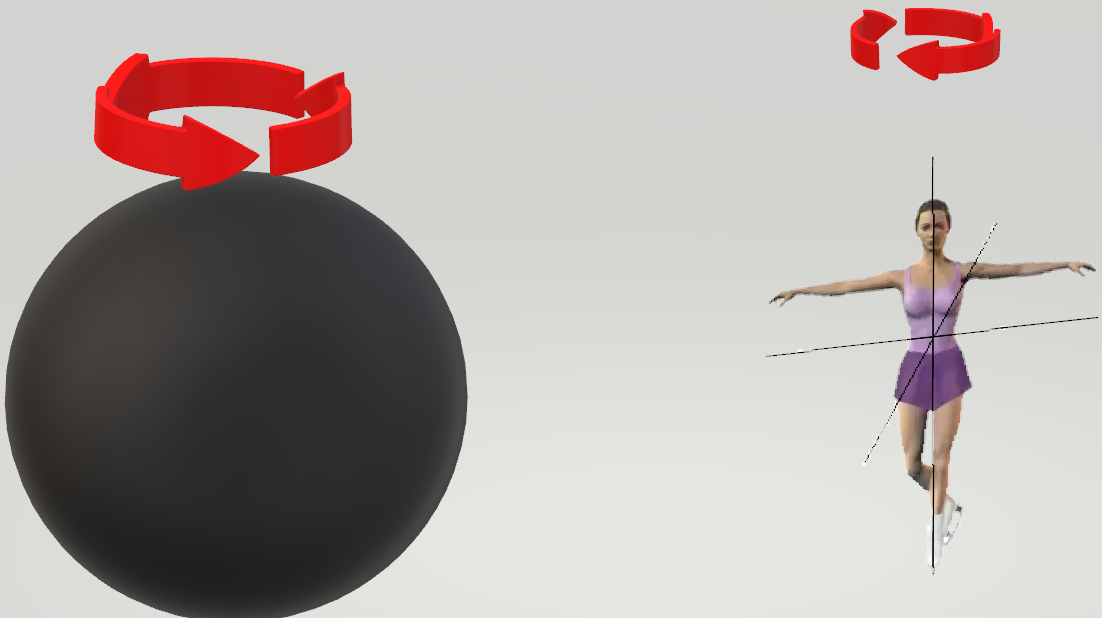
\includegraphics[width=\linewidth]{img/addison-wesley}
	\end{minipage}%
	\hfill
	\begin{minipage}{0.5\textwidth}
		\centering
		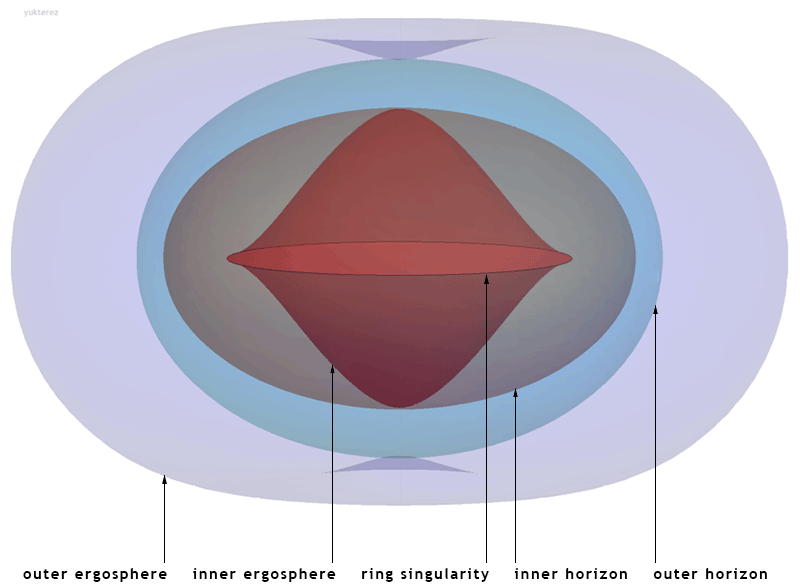
\includegraphics[width=0.9\linewidth]{img/Kerr-surfaces}
	\end{minipage}
	\caption{A model to help show the frame dragging effect (left). A diagram showing key regions and surfaces in the Kerr metric \cite{yukterezkerrnewman} (right).}
	\label{fig:Figure4.1}
\end{figure}

\section{Deriving the equations of motion}\label{sec:Section4.5}

	There are many formulations of the equations of motion of a particle/photon in the Kerr metric, a notable difference in complexity appears compared to those derived from the Schwarzschild metric in section \ref{sec:Section3.3}, this is because unlike the spherical symmetric which we took advantage of when working in the Schwarzschild metric, we now work in a metric with symmetry only about the axis of rotation. This symmetry does not simplify equations of motion much so we end up with the following, based upon \cite{yukterezKerr}:

\vspace{1em}
	Given initial position $(r, \theta, \phi)$, initial velocity v, spin parameter a, launch angle $\alpha$ and inclination angle $\delta$ one may use the Hamiltonian formalism as in section \ref{sec:Section3.3} to find velocities relative to a zero-angular momentum observer:
	
	\[v_r = v\sin(\alpha), v_\phi = v\cos(\alpha)\cos(\delta), v_\theta = v\cos(\alpha)\sin(\delta).\]

\vspace{1em}
	In the Kerr metric we see that the covariant metric coefficients are equal to:

	\[g_{tt} = 1-\frac{2r}{\Sigma},\]
	\[g_{t\phi} = g_{{\phi}t} = \frac{2ar\sin^2(\theta)}{\Sigma},\]
	\[g_{rr} = -\frac{\Sigma}{\Delta},\]
	\[g_{\theta\theta} = -\Sigma,\]
	\[g_{\phi\phi} = -\frac{\chi\sin^2(\theta)}{\Sigma}.\]

	And contravariant coeffiecients calculated by finding the inverse of the covariant matrix are:

	\[g^{tt} = \frac{\chi}{\Sigma\Delta},\]
	\[g^{t\phi} = g^{{\phi}t} = \frac{2ar}{\Sigma\Delta},\]
	\[g^{rr} = -\frac{\Delta}{\Sigma},\]
	\[g^{\theta\theta} = -\frac{1}{\Sigma},\]
	\[g^{\phi\phi} = -\frac{\Delta-a^2\sin(\theta)^2}{\Sigma\Delta\sin^2(\theta)}.\]

\vspace{1em}
	Then for our calculable initial conditions and constants, using proper time as our time-like variable $\tau$:

	\[\omega = \frac{2ar}{\chi} = \mbox{ Frame-dragging angular velocity,}\]
	\[L_{z} = v_{\phi}\sin(\theta)\sqrt{\frac{\chi}{\Sigma}} = \mbox{ Constant angular momentum along } \phi,\]
	\[E = \sqrt{\frac{\Delta\Sigma}{\chi}}+L_{z}\omega = \mbox{ Total energy (constant),}\]
	\[p_{\phi} = L_{z},\]
	\[p_{r} = v_{r}\sqrt{\frac{\Sigma}{\Delta}},\]
	\[p_{\theta} = v_{\theta}\sqrt{\Sigma},\]
	\[Q = {p_{\theta}}^2+\cos^2(\theta)\left(\frac{{L_{z}}^2}{\sin^2(\theta)}-a^2E^2\right) = \mbox{ Carter's constant },\]
	\[k = Q+{L_{z}}^2+a^2E^2 = \mbox{ Carter's k (constant).}\]

\vspace{1em}
	And for our system of first order differential equations (dot here represents differentiation with respect to proper time):

	\[\dot{r} = p_r\frac{\Delta}{\Sigma},\]
	\[\dot{\theta} = \frac{p_\theta}{\Sigma},\]
	\[\dot{\phi} = \frac{2arE\sin^2(\theta)+L_{z}\Sigma-2t}{\Sigma\Delta\sin^2(\theta)},\]
	\[\dot{p_{\phi}} = 0,\]
	\[\dot{p_{\theta}} = \frac{\sin(\theta)\cos(\theta)(L^2-a^2E^2\sin^4(\theta))}{\Sigma\Delta\sin^4(\theta)},\]
	\[\dot{p_{r}} = \frac{2rE^2(r^2+a^2)-k(r-1)-2aEL_{z}}{\Sigma\Delta}-\frac{2{p_{r}}^2(r-1)}{\Sigma}.\]

\vspace{1em}
	This is presented in as simple manner possible, and the order terms and equations are presented above are not the order in which they would be derived if we were to formally calculate them.
	

\section{Modelling a photon path}\label{sec:Section4.6}

	As mentioned above, we will be modelling the path of a photon in the Kerr metric using relativistic ray tracing. We will use solve\_ivp and solve along the variable proper time $\tau$.

\vspace{1em}
	Using this basis, we use solve\_ivp to generate a list of $r, \theta, \phi, p_{\phi}, p_{\theta}, p_{r}$, and from this we can plot the path of such a photon using Boyer-Lindquist coordinates (see figure \ref{fig:Figure4.2}).

\vspace{1em}
	The first thing that we will do is to find our launch angle and inclination angle for given pixel (i,j) on a HDRI image. By construction a HDRI image is 2x1 aspect ratio and the (i,j)$^{\mbox{th}}$ pixel corresponds to angles $\theta_x$, $\theta_y$ rotation about the y-z, x-z planes of the cameras coordinates respectively. A simpler way to think of this is that i is directly proportional to $\phi$, and j to $\theta$ in the usual three-dimensional polar coordinates (here with r = celestial sphere radius).

\vspace{1em}
	Via some elementary geometry, we can find the launch angle $\alpha$ - the angle between a line formed from our initial and final positions, and the cameras coordinate system's z-axis. And the inclination angle $\delta$ - the rotational angle required to transform the equatorial plane to a plane containing our initial and final positions, and the centre of the black hole (see figure \ref{fig:Figure3.2} (right)):

\vspace{1em}
	\[\alpha = \cos^{-1}(\cos(\theta_x)\cos(\theta_y)),\]
	\[\delta = \pi+\cos^{-1}\left(\frac{\sin(\theta_x)\cos(\theta_y)}{\sqrt{\sin^2(\theta_x)\cos^2(\theta_y)+\sin^2(\theta_y)}}\right)\mbox{ If j}\geq0\mbox{ and} \]
	\[\delta = \pi-\cos^{-1}\left(\frac{\sin(\theta_x)\cos(\theta_y)}{\sqrt{\sin^2(\theta_x)\cos^2(\theta_y)+\sin^2(\theta_y)}}\right)\mbox{ If j}<0.\]

\vspace{1em}
	A special case arises if (i,j) = (0,0), since we would be dividing by 0 in the calculation of $\delta$. Here we take launch and inclination angles to both be 0, though the inclination angle does not affect the path when the launch angle is 0.

\begin{figure}[!ht]
	\centering
	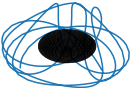
\includegraphics[width=0.3\linewidth]{img/kerr-path}
	\caption{A plot of a photon in the Kerr metric $\left( \mbox{initial conditions }r=3, \theta=\frac{\pi}{2}, \phi=0, v=1, a=1, \alpha=0, \delta=-\sin^{-1}(\frac{1}{3})\right)$.}
	\label{fig:Figure4.2}
\end{figure}

\section{Generating an image of the effects of gravitational lensing}\label{sec:Section4.7}

	Now that we have a method to find the final position in the Kerr metric given initial conditions, for each pixel in our image, we may numerically solve the coupled differential equations as in section \ref{sec:Section4.6}. If the solution status shows that an event took place  (i.e., the photon passed the event horizon), or the final radial position of the photon is within the ergoregion (likely a trapped path) we update the current pixel to black on a copy of our celestial sphere image. If not, we find the final point ($x_1,y_1,z_1$) of our photons path in the Cartesian coordinates describing the cameras coordinate system, and find the angles formed between a straight line from our initial position ($x_0,y_0,z_0$) to final position, with the x-z plane and the x-y plane, for a tuple directly proportional to the pixel coordinates of the final position on the original image.

\vspace{1em}
	Again, via elementary geometry, one may find that:

	\[\mbox{width}_{\mbox{angle}} = \tan^{-1}\left(\frac{x_1-x_0}{y_1-y_0}\right) (+\pi \mbox{ if } y_1<y_0),\]
	\[\mbox{height}_{\mbox{angle}} = -\tan^{-1}\left(\frac{z_1-z_0}{\sqrt{(x_1-x_0)^2+(y_1-y_0)^2}}\right).\]

\vspace{1em}
	After converting these angles to pixel coordinates by multiplying by $\frac{\mbox{height}}{\pi}$, then taking modulo width or height (if we are calculating the x or y pixel coordinate respectively). We can update our copy of the celestial sphere with the relevant final pixel position, and get an image such as figure \ref{fig:Figure4.3}, showing the effects of gravitational lensing caused by a Kerr black hole on a celestial sphere.

\begin{figure}[!ht]
	\centering
	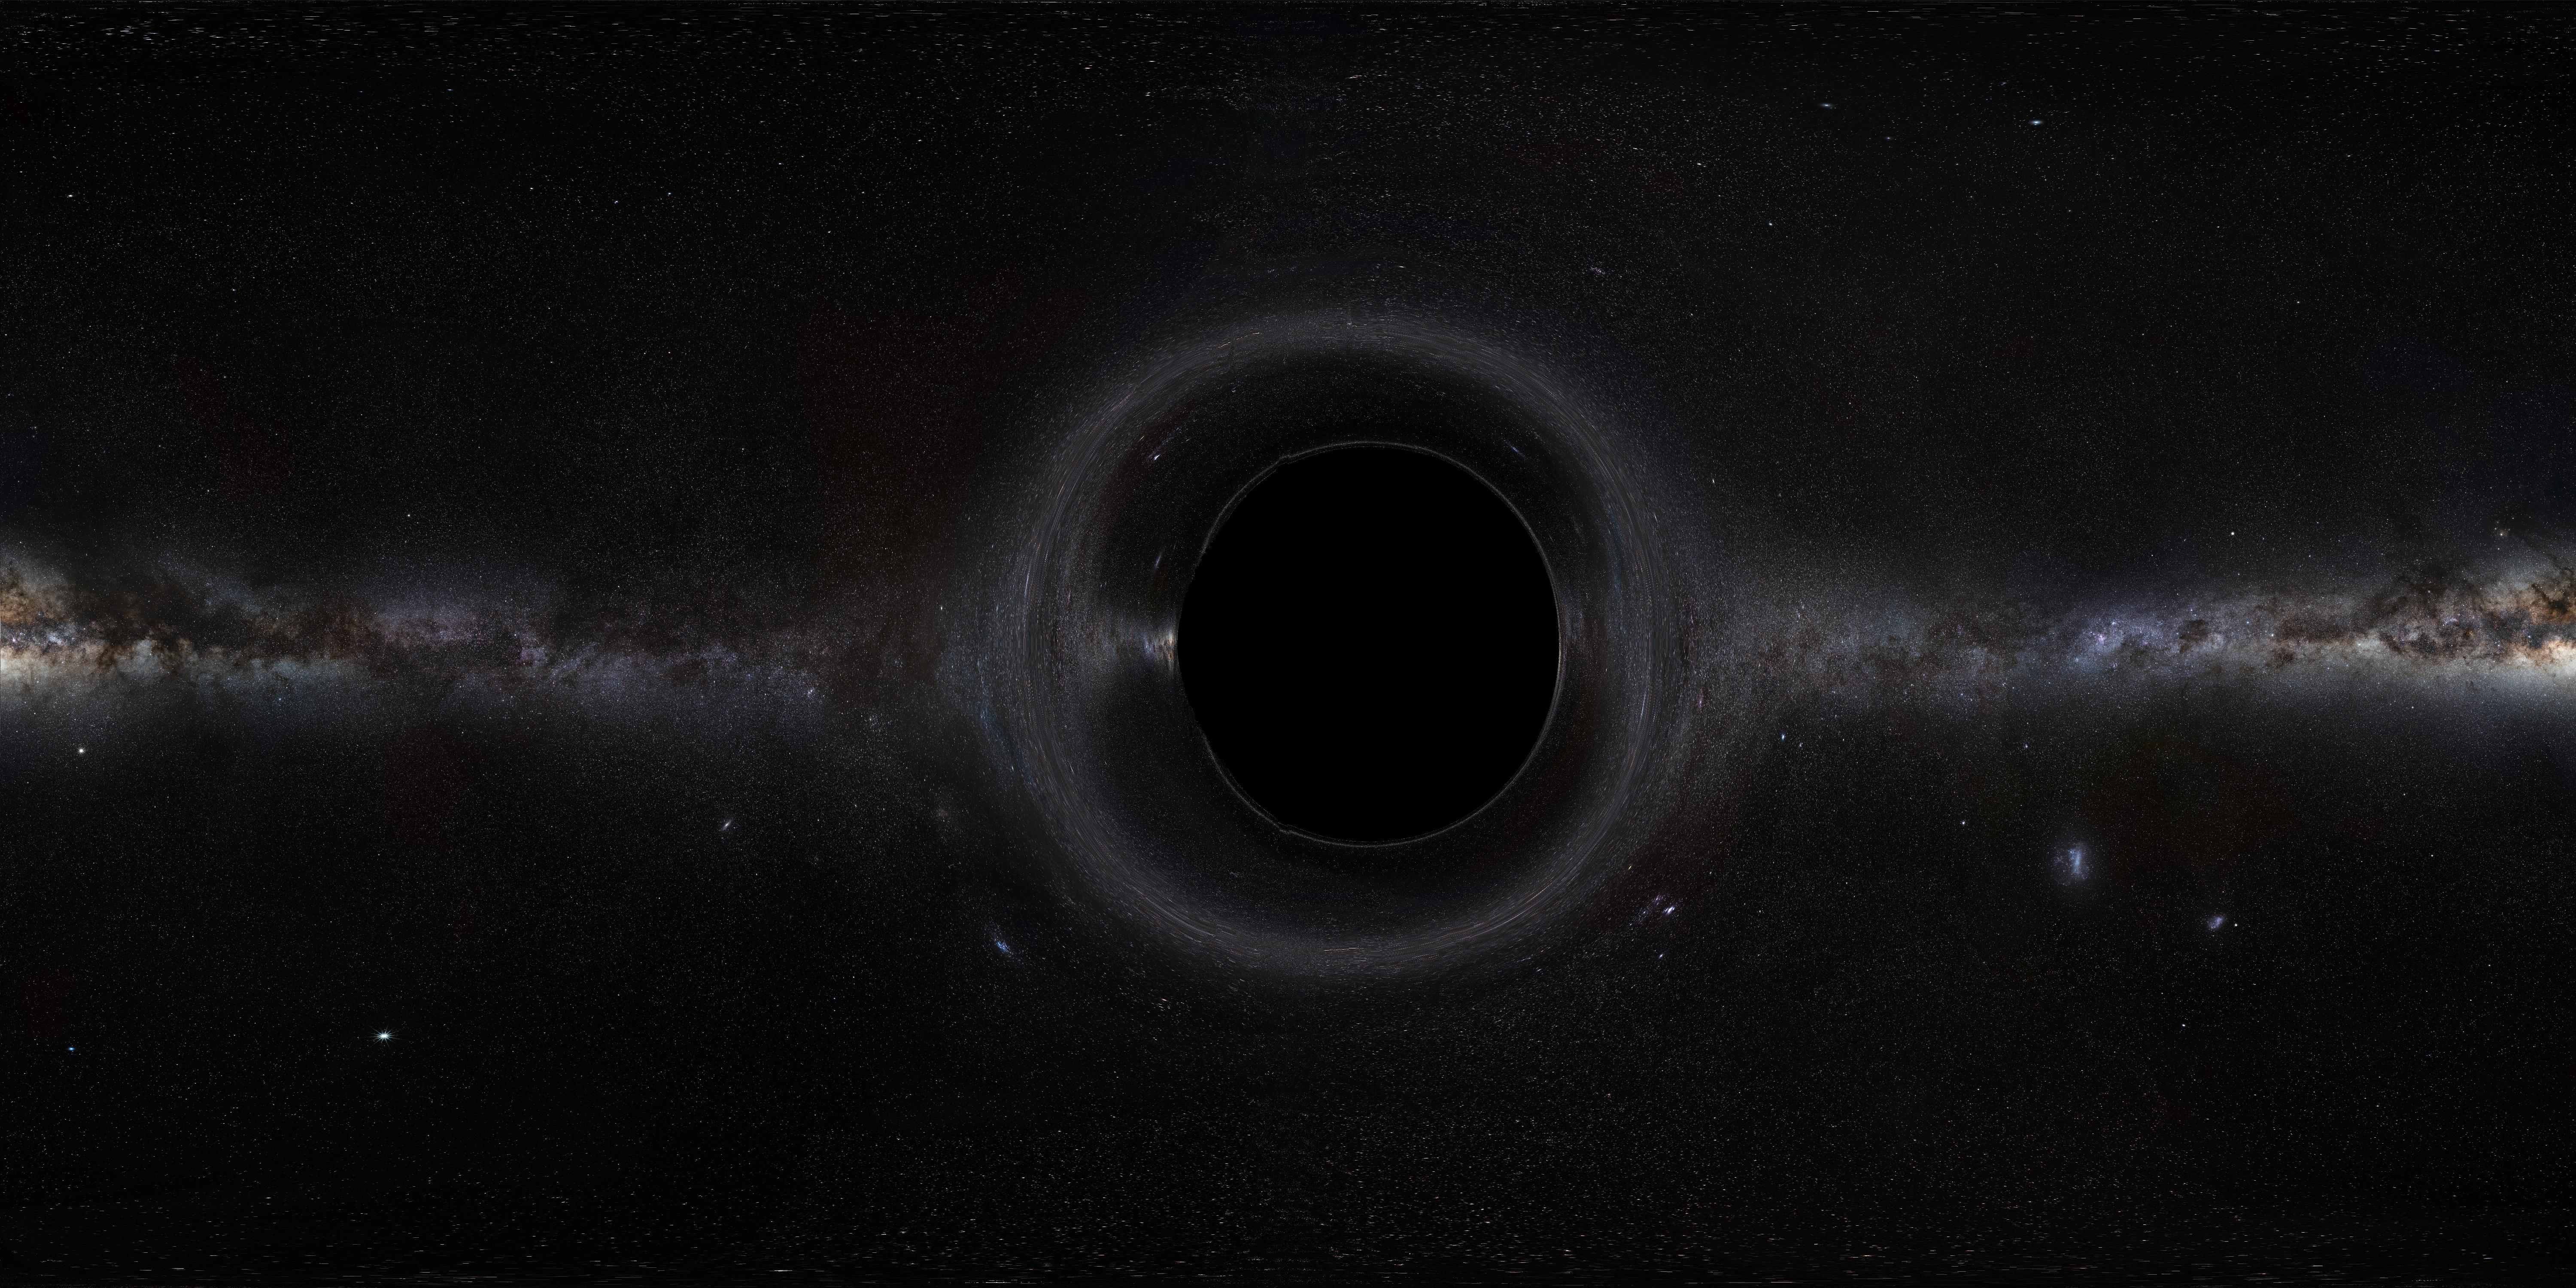
\includegraphics[width=\linewidth]{img/milkyway-kerr-full-new}
	\caption{A model of a Kerr black hole with spin parameter a=0.998.}
	\label{fig:Figure4.3}
\end{figure}

\section{Analysing the image}\label{sec:Section4.8}

	Looking carefully at figure \ref{fig:Figure4.3}, there are details which inform us of the nature of the Kerr metric, and how it affects light. In this section we will take a look at some of these characteristic details and what causes them. 

\subsection{Shadow caused by the event horizon}\label{subsec:Subsection4.8.1}

\vspace{1em}
	First and foremost of the notable characteristics of figure \ref{fig:Figure4.3} is the event horizon, as mentioned in chapter \ref{chap:Chapter1}, we see the shadow caused by the event horizon and its distinctive D-shape. The transformation from a central and circular shadow to this shape is smooth, as one would expect, as spin parameter increases from zero to one. This shape is explained by from the fact that a photon orbiting the black hole in the same direction as it's spin gains energy, and conversely a photon orbiting against the direction of spin loses energy in a manner similar to moving with or against the current of a river. Where a photon path in the Schwarzschild metric may cross the event horizon, if it is a prograde orbit (corotating with a Kerr black hole), in some circumstances it may escape. This leads to a flattened side on the shadow on the side of corotation, and similarly the opposite side is expanded.

\vspace{1em}
	As was the case with the images we generated of the gravitational lensing caused by a Schwarzschild black hole in chapter \ref{chap:Chapter3}, we can see various repeated images - with a particularly notable example near the flat edge of the shadow. The explanation as to the primary, secondary and so on images given in section \ref{sec:Section3.6} remains applicable in the Kerr metric, and the reasoning behind the clear example on the flat side is that due to the addition of spin, a photon is able to orbit the black hole many times more easily when corotating with the black hole than without spin; meaning the multiple images of the same band which would be visible in a perfect resolution image of the effects of a Schwarzschild black hole, are more easily seen here. 

\vspace{1em}
	There are very few pixels relating to retrograde paths (not co-rotating) which allow for multiple orbits and eventual escape of the black hole, given a perfect image and zooming capabilities we would still see an infinitely repeating pattern, though interestingly a very different pattern to those produced by prograde orbits as seen in \cite[pg. 8-11]{seeingRelativity}. However, on the opposite side of the picture, with pixels relating to prograde paths, there is a significantly larger area in which photons may orbit the black hole many times and escape due to the gained angular momentum.

\vspace{1em}
	Much of the repeating images on the flat side are caused by photon orbits which enter and exit the ergoregion. This is particularly the case due to the extremity of the spin parameter used; making the possible energy gained, and maximal distance between outer horizon and outer ergosphere, relatively large.

\vspace{1em}
	The size of the shadow is affected by relativistic aberration, an effect in special and general relativity caused by the speed of an observer. If an observer is moving at a considerable fraction of the speed of light, the captured image is very different to that of an observer at rest. Since we take a fiducial observer, which is not at rest, our image is representative only of an observer at rest rotationally. The more one corotates with a Kerr black hole, the less of its shadow one sees, meaning a totally at rest observer would see a larger, more distorted view of the black holes shadow.

\subsection{Caustics and critical curves}\label{subsec:Subsection4.8.2}

\vspace{1em}
	For images generated showing a celestial sphere with a Kerr black hole in front of it, we see critical curves, which are closed curves relating to all initial angles which reach a caustic curve without completing a full orbit of the black hole. A caustic curve is an analogue of the caustic point directly behind a Schwarzschild black hole with reference to the observers past light-cone, whose image is the Einstein ring. The primary caustic curve of an observer in the Kerr metric is the intersection between a two-dimensional caustic surface in the observers past light-cone, and the celestial sphere (see figure \ref{fig:Figure4.4} (right)). Caustics are closed curves for Kerr black holes, rather than a point directly behind the black holes centre in line with the camera, as is the case in the Schwarzschild metric. The primary critical curve is not circular in figure \ref{fig:Figure4.3}, but rather a rounded rectangular shape, and can be clearly seen in figure \ref{fig:Figure4.3} as the distortion of the milkyway, which lies directly behind the black hole.

\vspace{1em}
\begin{figure}[!ht]
	\centering
	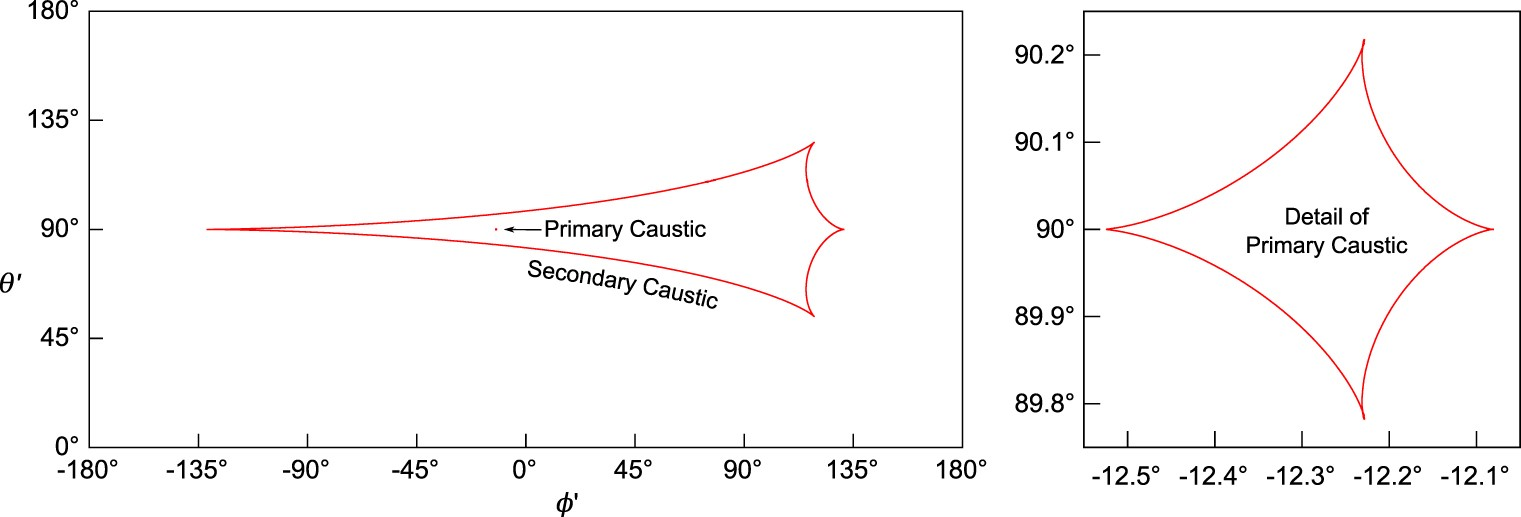
\includegraphics[width=0.87\linewidth]{img/caustic0}
	\caption{An figure showing primary and secondary caustics as found in \cite{thorne2015gravitational}, note that this is case by case and does not necessarily represent the caustics for figure \ref{fig:Figure4.3}. Credit to DNEG for original image}
	\label{fig:Figure4.4}
\end{figure}

\vspace{1em}
	There is also a secondary critical curve, which is the same as the primary critical curve, but generated by the secondary caustic, which is a significantly larger curve than the primary caustic, and stretched in the $\phi$-direction (see figure \ref{fig:Figure4.4} (left)). The secondary critical curve can be seen as the closed curve relating to all initial angles which reach the primary caustic curve, but with one orbit in transit. Each time you cross a critical curve on an image the direction of motion of what is viewed flips, if we were to produce an animation from an orbiting camera, we would see that the direction of motion for stars on the image switches each time we cross a critical curve. We see this behaviour in figure \ref{fig:Figure4.5} as the direction of the movement of stars is flipped as we enter the primary critical curve.

\vspace{1em}
	Critical curves cause some very interesting behaviour, including the creation, and annihilation of stellar image pairs. As a star's position on our celestial sphere changes, it may cross a critical curve, each time a light source crosses a critical curve, a stellar image pair is either created or annihilated; that is to say that one new image of the star will either be formed, or destroyed inside the curve on our model. 

\vspace{1em}
	At the moment of creation and annihilation, the relative intensity of the star and it's new image spikes dramatically, causing creation and annihilation to be noticeable in animations \cite{thorne2015gravitational}.

\vspace{1em}
\begin{figure}[!ht]
	\centering
	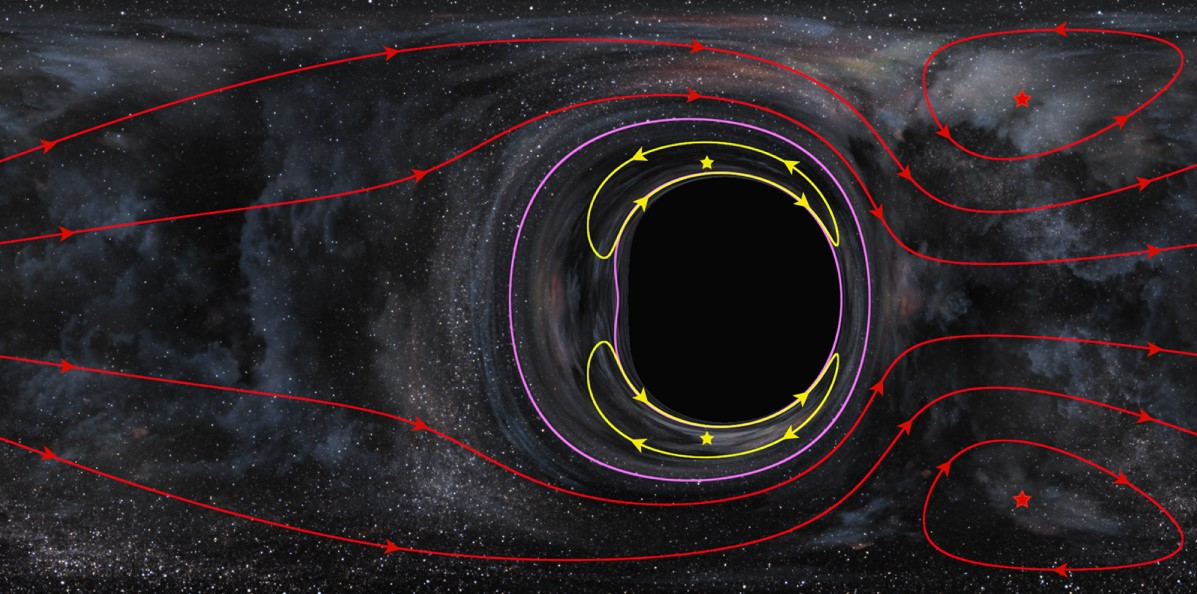
\includegraphics[width=0.87\linewidth]{img/caustic}
	\caption{An image showing the primary paths of light sources (red), the paths of their secondary images (yellow), and the primary (outer) and secondary (inner) critical curves (purple). Copyright ©  2015 Warner Bros. Entertainment Inc. Interstellar}
	\label{fig:Figure4.5}
\end{figure}

\subsection{Testing our accuracy}\label{subsec:Subsection4.8.3}

	In this section, we run our code using a celestial sphere as used in \cite{thorne2015gravitational}; a checkerboard of paint. This serves to provide a check to see if our code is running as it should, and allows us to use a very clear picture to show how gravitational lensing affects the original image, as each final patch can be traced clearly to its origins on the original picture (see figure \ref{fig:Figure4.6} (right)).

\vspace{1em}
\begin{figure}[!ht]
	\centering
	\begin{minipage}{0.5\textwidth}
		\centering
		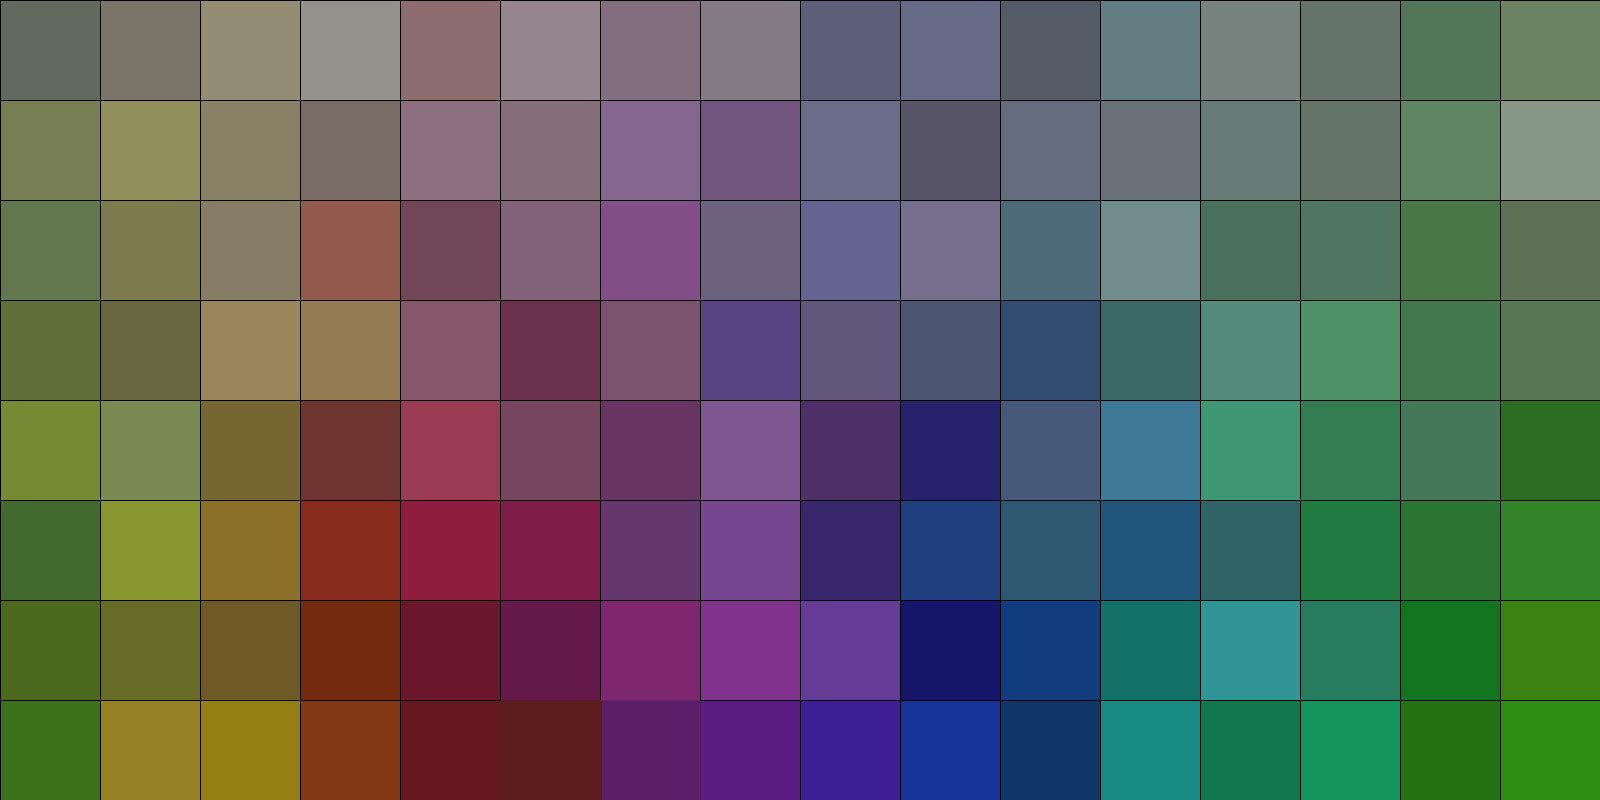
\includegraphics[width=0.95\linewidth]{img/checkerboard-own}
	\end{minipage}%
	\hfill
	\begin{minipage}{0.5\textwidth}
		\centering
		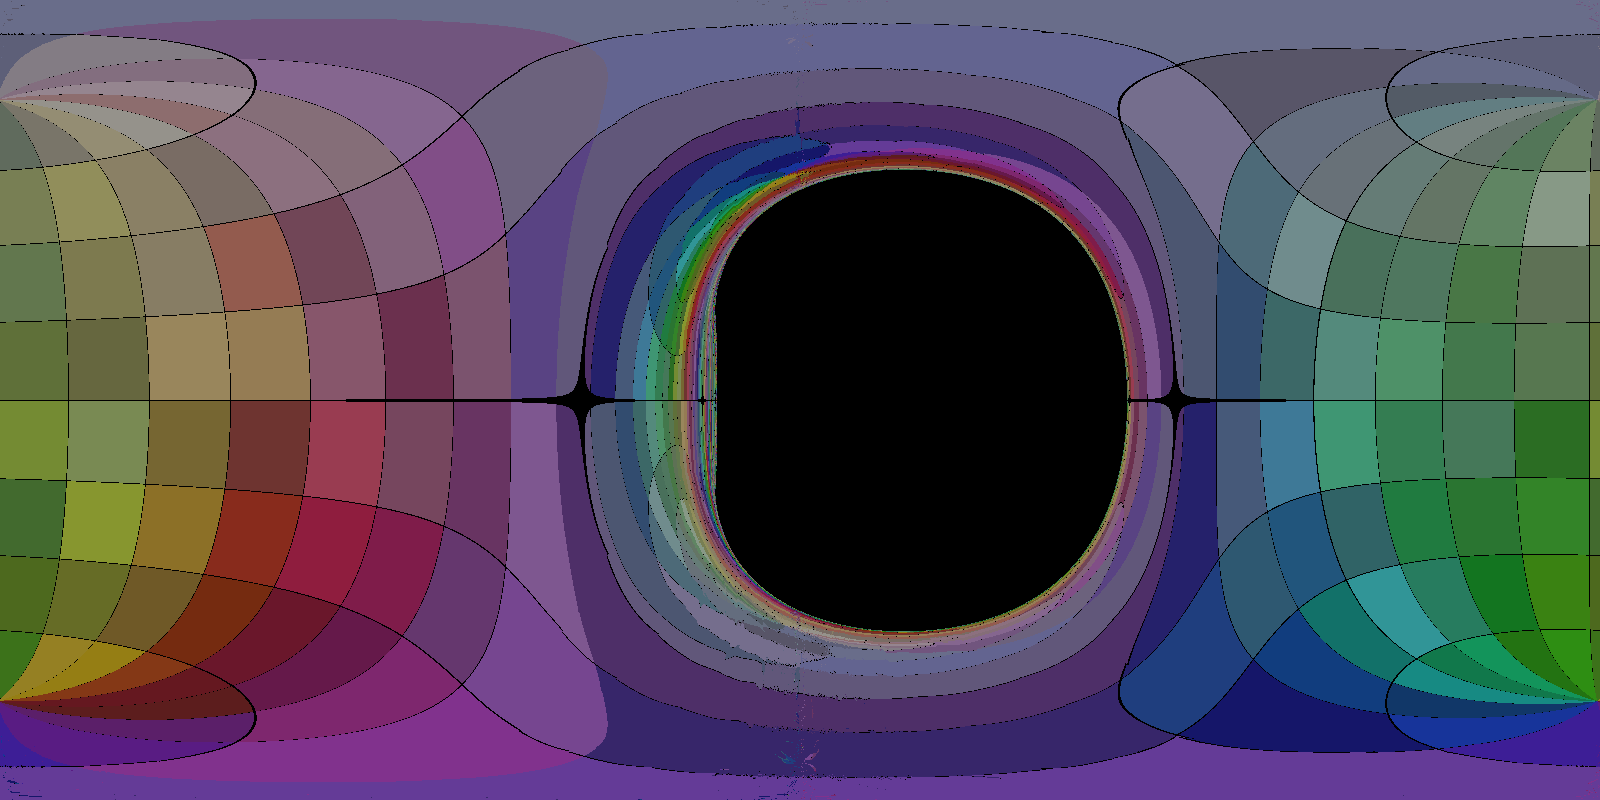
\includegraphics[width=0.95\linewidth]{img/checkerboard-own-kerr}
	\end{minipage}
	\caption{A coloured checkerboard (left). A model showing the effects of gravitational lensing on a coloured checkerboard (right).}
	\label{fig:Figure4.6}
\end{figure}

\vspace{1em}
	The result of this test was an almost one-to-one image, which shows our code is running well, at least on a cursory glance. Rather unsurprisingly we see that the more central a colour is, the more space it takes up in the final image, this is because there are many relatively 'easy' paths a photon can take to reach more central colours.

\vspace{1em}
	Using our working model, we will seek to improve and add to what we have in the aim of generating a more realistic image for astrophysical black holes as would theoretically be observed in the universe. This is what we will work towards in the next chapter.




\chapter{Generating a more realistic image}\label{chap:Chapter5}

	Now that we have an accurate model showing the gravitational lensing caused by a Kerr black hole, we can begin to consider effects and properties to improve the realism of our currently idealised model.

\section{Accretion discs}\label{sec:Section5.1}

	Given what we know of black holes in the universe, in all likelihood most if not all active black holes are surrounded by matter which orbits the singularity and continuously moves towards the event horizon, 'feeding' the black hole. This matter is known as an accretion disc, and there are various methods one can use to model them.

\vspace{1em}
	The simplest model for an accretion disc is a flat annulus on the equatorial plane of the black hole, we can keep track of if a photon path intersects with this annulus and if so, use a png to map the final pixel to launch pixel. This is the most common but unrealistic method of modelling, and gives us a good general idea as to what an accretion disc looks like from an observer's standpoint. This kind of model can be used to form an image using the same ideas as figure \ref{fig:Figure4.4}, with a test accretion disc to show explicitly what the effects of gravitational lensing on an accretion disc are (see figure \ref{fig:Figure5.1}). Given the limited length of this paper we will use this model moving forwards but we discuss more realistic models for those interested.


\vspace{1em}
\begin{figure}[!ht]
	\centering
	\begin{minipage}{0.5\textwidth}
		\centering
		
\includegraphics[width=0.9\linewidth]{img/test-accretion}
	\end{minipage}%
	\hfill
	\begin{minipage}{0.5\textwidth}
		\centering
		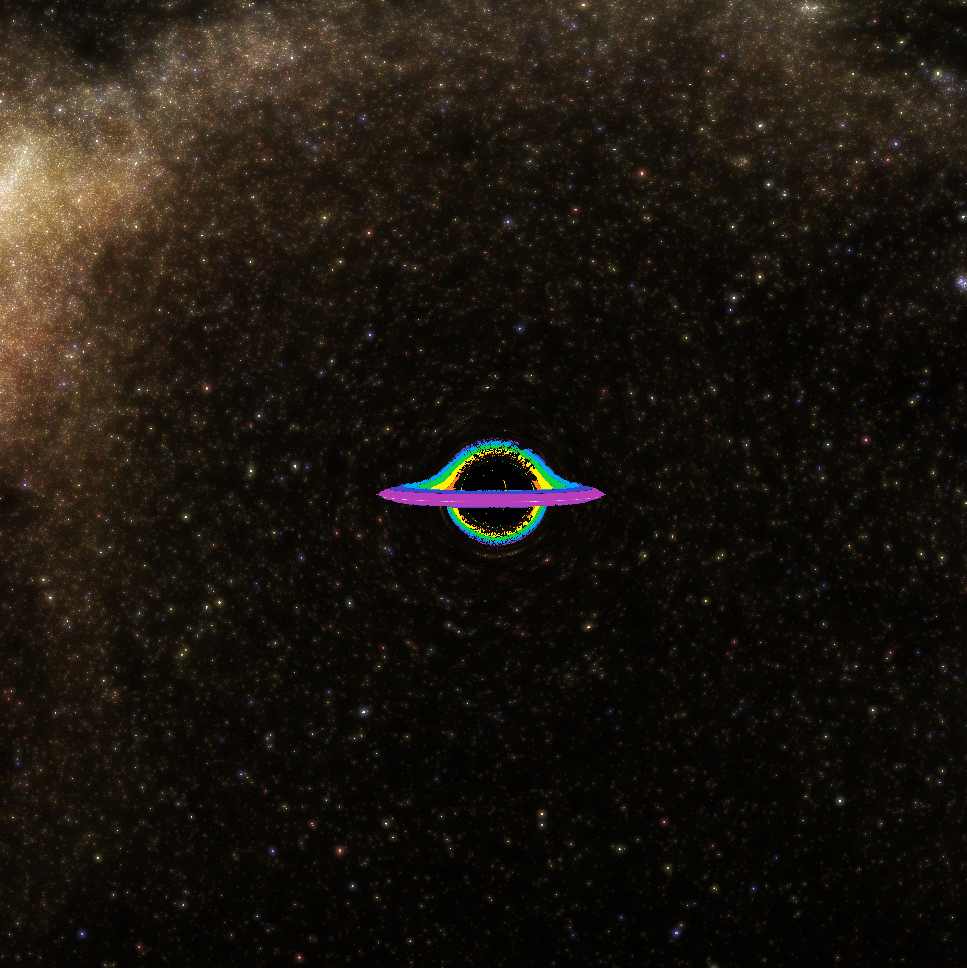
\includegraphics[width=0.9\linewidth]{img/milky-way-hdri-accretion(1)}
	\end{minipage}
	\caption{A test accretion disc (left). A model generated using a test accretion disc to show how an accretion disk affects the model (right).}
	\label{fig:Figure5.1}
\end{figure}

\vspace{1em}
	A much more realistic method is to model the accretion disc as a gas-like energy with an accretion rate which affects the energy flux. This is a thin relativistic accretion disc and the effects covered in section \ref{sec:Section5.2} can be easily applied. Interestingly the first, 'simple', approach is a good approximation to this method when taking the disc not to be accreting energy, as was the model for the film Interstellar. This method was used by Jean-Pierre Luminet to find apparent (bolometric) flux at various radii around a Kerr black hole and create the first 'image' of an accretion disc based upon mathematics.

\vspace{1em}
	In reality, it would be very unlikely to find a non-accreting accretion disc, this is because the rapid rotating near the inner ring causes a large amount of friction; and hence energy to be accreted.

\vspace{1em}
	We will now give a summary of a paper by Thorne and Novikov\cite{novikov1973astrophyics} giving insight into a more realistic model of an accretion disc and how one may derive the equations governing it. If one makes certain assumptions pertaining to the behaviour of an accretion disc, then in tandem with the laws of conservation (of mass, angular momentum, and energy) one may derive equations defining a more complex model for an accretion disc. First, we will start with a summary of the assumptions made:

\vspace{1em}
\begin{itemize}
	\item The central plane of the disk lies on the equatorial plane of the metric.
	\item At radius r, the disc is much thinner than the absolute value of r.
	\item There exists a time period which is not substantial enough for the external geometry of the metric to change significantly, but is large enough that the inward flow of mass in any region of interest is large when compared to the normal mass in this region.
	\item After being averaged over time, $\phi$, and height, the baryons move practically in equatorial, circular, geodesic orbits around the centre of the black hole.
	\item Heat flow within the accretion disc is only non-negligible for the vertical direction (normal to the equatorial plane).
	\item The only stress-energy from the accretion disc which reaches an observer is carried by photons (so no gravitational or magnetic energy is of relevance to us).
	\item One may neglect any energy transfer from one region of the accretion disc to another (this assumption is our most unreasonable assumption, as energy passing from the inner region of the disc will naturally transfer energy as it passes through).
\end{itemize}

\vspace{1em}
	We then obtain general equations defining an accretion disc model in a suitably symmetric metric (the Kerr metric satisfies this requirement):

\vspace{1em}
	\[\dot{\mbox{M}}_0 = -2ru^r\pi\Lambda,\]
	\[\mbox{F}_s = \frac{\dot{\mbox{M}}_0}{4r\pi}f,\]
	\[{\mbox{W}^{\phi}}_r = -\frac{\dot{\mbox{M}}_0(E^\dag-L^\dag\Omega)}{2r\pi\Omega_{,r}}f,\]
	\[f = -\frac{\Omega_{,r}}{(E^\dag-L\Omega^\dag)^2}\int_{r_{ms}}^{r} (E^\dag-L^\dag\Omega){L^\dag}_{,r} \,dr.\]

\vspace{1em}
	Where $\Lambda$ is the time averaged surface density of baryons on the disc, and using the notation of comma followed by a variable in subscript to denote partial differentiation with respect to the proceeding variable. $E^\dag$, $L^\dag$ and $\Omega$ are specific energy at infinity, specific angular momentum and angular velocity respectively. ${\mbox{W}^{\phi}}_r$ is defined to be $\sqrt{g^{rr}}$ multiplied by the time-averaged torque per unit circumference acting on a cylinder at radius r. Note that $g^{rr}=-\frac{\Delta}{r^2+a^2\cos^2(\theta)}$ in the Kerr metric.

\vspace{1em}
	Also here $r_{ms}$ is the inner radius of marginal stability found by imposing stability on bound circular orbits about the metric, specifically we impose that $\frac{dE^\dag}{dr}=\frac{dL^\dag}{dr}=0$.

\vspace{1em}
	Here $\dot{\mbox{M}}_0$ is the time averaged, radially independent rate at which mass flows inward through the accretion disc. Also, r and a are as we have seen them throughout this paper, and the intrinsic flux is a scalar due to the fact that it represents the time averaged flux of radiating energy flowing out of the upper face of the accretion disc (measured by an observer above the equatorial plane who is orbiting along with the time averaged motion of the accretion disc). u(r) is defined to be the mass and time averaged 4-velocity of the baryons.

\vspace{1em}
	When specifically applying such a model to the Kerr metric, one finds that:

\vspace{1em}
\begin{dmath}
	\mbox{F}_s = \frac{3\dot{\mbox{M}}_0}{8r\pi(r^{\frac{3}{2}}-3r^{\frac{1}{2}}+2a)}\left(r^{\frac{1}{2}}-x_0-\frac{3a}{2}\mbox{log}\left(\frac{r^{\frac{1}{2}}}{x_0}\right)-\frac{3(x_1-a)^2}{x_1(x_1-x_2)(x_1-x_3)}\mbox{log}\left(\frac{r^{\frac{1}{2}}-x_1}{x_0-x_1}\right)-\frac{3(x_2-a)^2}{x_2(x_2-x_1)(x_2-x_3)}	\mbox{log}\left(\frac{r^{\frac{1}{2}}-x_2}{x_0-x_2}\right)-\frac{3(x_3-a)^2}{x_3(x_3-x_1)(x_3-x_2)}\mbox{log}\left(\frac{r^{\frac{1}{2}}-x_3}{x_0-x_3}\right)\right).
\end{dmath}

\vspace{1em}
	With

	\[a = \mbox{positive spin},\]
	\[Z_1 = 1+(1-a^2)^{\frac{1}{3}}\left((1+a)^{\frac{1}{3}}+(1-a)^{\frac{1}{3}}\right),\]
	\[Z_2 = (3a^2+{Z_1}^2)^{\frac{1}{2}},\]
	\[x_0 = (3+Z_2-\left((3-Z_1)(3+Z_1+2Z_2)^{\frac{1}{2}}\right)^{\frac{1}{2}},\]
	\[x_1 = 2\cos\left(\frac{1}{3}\cos^{-1}(a)-\frac{\pi}{3}\right), x_2 =2\cos\left(\frac{1}{3}\cos^{-1}(a)+\frac{\pi}{3}\right) , x_3 = -2\cos\left(\frac{1}{3}\cos^{-1}(a)\right),\]

\vspace{1em}
	For ease of notation, x$_0$ (and so the Z's) are defined such that ${x_0}^2$=$r_{\mbox{ms}}$. The roots of the cubic equation x$^3$-3x+2a=0 are taken to be x$_1$, x$_2$ and x$_3$.

\vspace{1em}
	If one were seeking to use a more realistic model, in Astrophysics of Black Holes\cite{novikov1973astrophyics} Thorne and Novikov took the $\alpha$-disc model by Shakura and Sunyaev\cite{shakura1973black} and took into account relativistic effects to create an explicit formulation of an accretion disc consisting of an inner, middle and outer region. This allows for a complex and adaptive model of a relativistic accretion disc. This model however is computationally challenging and tends to only be used for the purpose of modelling realistic accretion discs.

\vspace{1em}
	For a more informative image of an accretion disc (see figure \ref{fig:Figure5.1} (right)), we will need to 'take a step back' and tilt upwards, meaning we will be placing our observer significantly further away than previously, and raising them about 10 degrees above the equatorial plane, this is to allow the observer to see an appropriately sized accretion disc without half the image being taken up by the accretion disc itself (if the observer were directly above the accretion disc).

\section{Relativistic effects}\label{sec:Section5.2}

	Mentioned several times already in this paper, any truly realistic relativistic model accounts for Doppler shift and aberration, these are naturally occurring phenomena which affect our accretion discs image greatly.

\subsection{Doppler shift}\label{subsec:Subsection5.2.1}

	Most readers will be aware of Doppler shift on a non-relativistic level, and certainly have experienced it. Doppler shift is the apparent changing of frequency of emitted energy due to the motion of the energy source. The most common example being an emergency services vehicles siren sounding higher pitched when incoming and lower pitched when moving away from the observer.

\vspace{1em}
	In non-relativistic Doppler shift, a medium (such as air) in which the waves propagate must exist, and the effects of time-dilation as considered in special relativity are negligible - as non-relativistic Doppler shift must be in a scenario not requiring a relativistic point of view.

\vspace{1em}
	In relativistic Doppler shift however, no medium of propagation is required, and the effect is caused by time-dilation due to energy sources moving at close to the speed of light. This of course is the case for our accretion disc, which is rotating extremely rapidly, particularly close to the event horizon.

\vspace{1em}
	On top of the relativistic Doppler effect, another cause of the shifting of frequencies our scenario calls us to consider would be gravitational redshift; in which a gravitational well causes a loss of energy, which corresponds to a loss of frequency. These effects occur to electromagnetic radiation and photons, but we are solely focussed on the effects on a generated image, meaning the effect it has on photons.

\vspace{1em}
	Gravitational redshift would affect all light sources in our image, granted, the accretion disc most extremely due to its proximity to the event horizon but for a most realistic image the effect should be considered for the entire picture - unlike the relativistic Doppler effect.

\vspace{1em}
	As well as redshift, relativistic Doppler shift also causes a shift in intensity of light, meaning photons which are blue shifted usually appear more intense, and photons which are redshifted are less intense. This is because as the frequency of the light increases or decreases, but the inherent energy stays the same, the energy flux increases or decreases along with the frequency. 

\vspace{1em}
	One commonly used method to account for intensity shift is implied by Liouville's theorem, which states that any bounded entire function must be constant. This, combined with the fact that $\frac{\mbox{the source intensity}}{\mbox{the source frequency cubed}}$ is a Lorentz invariant implies that the intensity is multiplied by the fourth power of the Doppler factor calculated for frequency shift discussed above.

\subsection{Aberration}\label{subsec:Subsection5.2.2}

	Another key relativistic effect which could significantly affect a system such as the one we are modelling is aberration. When an observer moves at a significant proportion of the speed of light; the intensity and amount of energy they receive from a source can be changed. Put in simpler terms, when an observer is moving towards an energy source, they move into some of the emitted energy; this means that the field of view can often be expanded, since energy which would under ordinary circumstances be unobservable is reached.

\vspace{1em}
	In section \ref{sec:Section4.4}, we had the foresight to change our metric to convert into a system with a fiducial observer, this actually removes any considerable effects caused by aberration as we are locally stationary. If we were stationary with respect to the original metric, depending on how close to the black hole we get; we would have to be 'moving' significantly against the rotation of the metric to counteract its effect on the space around. This can cause relativistic aberration, and since for many of our models we take the camera to be relatively close to the black hole this would be a factor to consider had we not performed the coordinate shift.

\section{A realistic image}\label{sec:Section5.3}

	We now have the components necessary to generate our final image, this is by no means perfect, and as mentioned in the previous few sections there are significantly more realistic methodologies when modelling accretion discs and dealing with relativistic effects. However, this is as realistic as we have time to explore, and is more realistic than the majority of portrayals in media, including Interstellar. 

\vspace{1em}
	In \cite{thorne2015gravitational} a realistic Kerr black hole is presented (see figure \ref{fig:Figure5.2} (right)), but Kip Thorne notes that Christopher Nolan wanted to balance realism with visual spectacle, so unfortunately although the film is touted as being remarkably scientifically accurate; the depiction of the black hole does not appropriately account for relativistic effects to be considered a realistic model.

\vspace{1em}
\begin{figure}[!ht]
	\centering
	\begin{minipage}{0.5\textwidth}
		\centering
		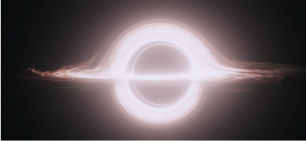
\includegraphics[width=0.9\linewidth]{img/used-kerr}
	\end{minipage}%
	\hfill
	\begin{minipage}{0.5\textwidth}
		\centering
		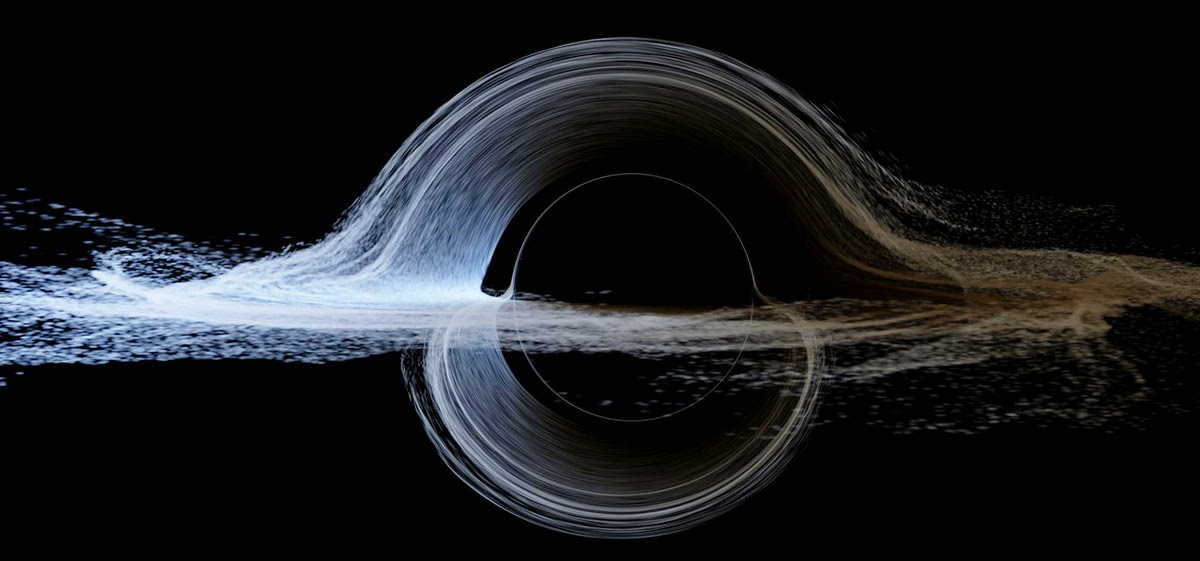
\includegraphics[width=0.9\linewidth]{img/realistic-kerr}
	\end{minipage}
	\caption{A still from the film Interstellar showing the black hole Gargantua (left). An accurate model of a Kerr black hole (right). (Credit for image to DNEG \& Warner Bros)}
	\label{fig:Figure5.2}
\end{figure}

\vspace{1em}
	Figure \ref{fig:Figure5.2} (right) shows a Kerr black hole with a non-accreting accretion disc, with gravitational redshift, Doppler frequency shift and Doppler intensity shift all accounted for; outside of the time saving simpler method of modelling the accretion disc, this is a very realistic depiction of what an observer would see.





\chapter{Using the Kerr metric to model a wormhole}\label{chap:Chapter6}

	We have a few metrics available to us for modelling a wormhole, all of which are very unstable with respect to gravitational perturbations. The most commonly used models are the Morris-Thorne wormhole, and a maximal analytic extension of the Kerr metric. In this chapter we will explore the mathematics of maximal analytic extensions, and analyse the findings of Alain Riazuelo in his recent paper on falling into a Kerr black hole\cite{seeingRelativity}.

\section{Maximal analytic extensions}\label{sec:Section6.1}

	To formulate the definition of a maximal analytic extension we define a manifold and geodesic completeness:

\vspace{1em}
	A manifold, or n-manifold is a space for which each point is homeomorphically equivalent to an n-dimensional subset of Euclidean space in a neighbourhood around it.

\vspace{1em}
	Formally a manifold is geodesically complete if the exponential map is defined at every point p on T$_p$(M): the tangent space at p. The exponential map of a metric defining an affine connection is given by the exponential map of this connection. Geometrically, a manifold is geodesically complete if every geodesic contained within can be extended arbitrarily.

\vspace{1em}
	Given two differentiable manifolds with analytic transition maps (analytic manifolds) $\mathfrak{M}$, $\mathfrak{M}'$ with $\mathfrak{M} \subset \mathfrak{M}'$ we call $\mathfrak{M}'$ a maximal analytic extension of $\mathfrak{M}$ if every geodesic of $\mathfrak{M}'$ is either complete or terminates at a singular point.

\vspace{1em}
	Often, maximal analytic extensions of metrics which are gravitationally stable and hence reasonable to model real phenomena, end up being unstable. This is the case for the extensions of the Schwarzschild and Kerr metric. However, there is still merit in analysing these metrics, as they describe areas unavailable to us ordinarily. It is worth moving forward with the fact that much of the analysis ahead is mostly mathematical, and so may be unreasonable physically.

\subsection{Extending the Schwarzschild metric}\label{subsec:Subsection6.1.1}

\vspace{1em}
	As Boyer and Lindquist did in their paper on maximal analytic extensions\cite{boyer1967maximal} we start by creating a non-maximal analytic extension of the Schwarzchild metric as coordinate transformations are very natural and the purpose is self-evident. We choose the coordinates $r=\bar{r}$, $\theta=\bar{\theta}$ and $\phi=\bar{\phi}$ with the 'bar' coordinates original Schwarzschild coordinates such that:

	\[dt = d\bar{t}+2m\frac{d\bar{r}}{\bar{r}-2m}.\]

\vspace{1em}
	This is a formulation of the Schwarzschild metric without the coordinate singularity at r=2m associated with the Schwarzschild coordinates. However, this metric is not geodesically complete for t$\rightarrow-\infty$, we may 'sew' this metric together with a similar metric with:

	\[dt = d\bar{t}-2m\frac{d\bar{r}}{\bar{r}-2m},\]

	to obtain a maximal form of the Schwarzschild metric for all r>0. However, although there is no physical representation, a maximal analytic extension must cover r<0, and so this formulation of the Schwarzschild metric is not a maximal analytic extension.

\vspace{1em}
	We will now provide a maximal analytic extension of the Schwarzschild metric; the first maximal analytic extension of the Schwarzschild metric was discovered by John Synge in 1950\cite{synge1950gravitational}, and was independently rediscovered by Szekeres\cite{szekeres1960singularities} and Kruskal\cite{kruskal1960maximal}. The latter papers providing much simpler coordinates that the former, and so are most commonly used, we now define Kruskal-Szekeres coordinates to acquire the maximal analytic extension of the Schwarzschild metric by replacing t, r in ordinary coordinates by T, X:

	\[T=(|\frac{r}{2}-1|e^{\frac{1}{2}})^{\frac{1}{2}}\sinh\left(\frac{t}{4}\right),\]
	\[X=(|\frac{r}{2}-1|e^{\frac{1}{2}})^{\frac{1}{2}}\cosh\left(\frac{t}{4}\right)\]

\vspace{1em}
	for r$\neq$2. We also see that we may define T, X as the (unique) solution to the equation:

	\[T^2-X^2 = \left(1-\frac{r}{2}\right)e^{\frac{r}{2}},\mbox{ } T^2-X^2<1.\]

\vspace{1em}
	We may now provide a well-defined transformation between the coordinates by:

	\[r = 2\left(1+W_0\left(\frac{X^2-T^2}{e}\right)\right),\]
	\[t = 4\tanh^{-1}\left(\frac{T}{X}\right) \mbox{ if }T^2-X^2<0 \mbox{ and } X>0),\]
	\[t = 4\tanh^{-1}\left(\frac{X}{T}\right) \mbox{ if }0<T^2-X^2<1) \mbox{ and } T>0\]

	where $W_0$ is the 0-branch of the Lambert $W$ function. In these coordinates, the Schwarzschild manifold is given by:

	\[g = \frac{32}{r}e^{-\frac{r}{2}}(-dT^2+dX^2)+r^2(d\theta^2+\sin^2(\theta)d\phi^2).\]

\vspace{1em}
	The only singularities we encounter when using these coordinates lie at r=0 $\Rightarrow$ T$^2$+X$^2$=1, and so particularly the event horizon r=2 is well defined. We defined a transformation between Kruskal-Szekeres coordinates and Schwarzschild coordinates, well-defined for r>2, -$\infty$<t<$\infty$, and can then extend this transformation up to r=0, meaning the above metric is a solution to Einstein field equations in this region. 

\vspace{1em}
	We conclude that we are left with a maximal analytic extension of the Schwarzschild metric, as noted by Kruskal, if one manually follows any geodesic in whichever direction, it will end at r=0, or is continuable infinitely (hence the coordinates lead to a maximal extension).

\vspace{1em}
	A Carter-Penrose diagram can be used to give a visual representation of the causal structure of the maximal analytic extension of a metric (see figure \ref{fig:Figure6.2}), a Carter-Penrose diagram is a two-dimensional diagram which is locally conformal to the metric each section describes. A Carter-Penrose diagram takes a two-dimensional subset (including time) of our four-dimensional spacetime, and maps it to two dimensional space to see some causal relation between the variables of this subsection.

\vspace{1em}
	For the Kruskal-Szekeres coordinates, the two-dimensional section we are interested in is spanned by U = T-X and V = T+X. Then using a mapping similar to the inverse of stereographic projection, we define $-\pi\leq\Psi,\Phi\leq\pi$ such that:

	\[U = \tan\left(\frac{\Phi-\Psi}{2}\right),\]
	\[V = \tan\left(\frac{\Phi+\Psi}{2}\right).\]

\vspace{1em}
	Then, by conformally affecting such a mapping, we may move an image such as the left of figure \ref{fig:Figure6.1}, to the image on the right (the conformal shift being to acquire straight lines for r=0). Now we have our Carter-Penrose diagram, and may analyse it.

\vspace{1em}
\begin{figure}[!ht]
	\centering
	\begin{minipage}{0.5\textwidth}
		\centering
		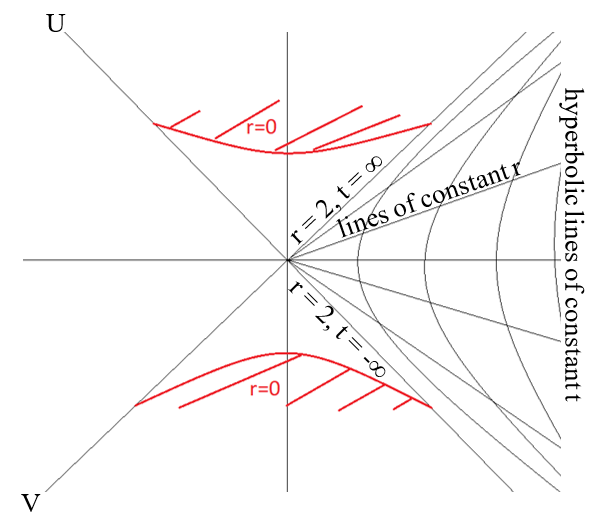
\includegraphics[width=0.9\linewidth]{img/carter-penrose1}
	\end{minipage}%
	\hfill
	\begin{minipage}{0.5\textwidth}
		\centering
		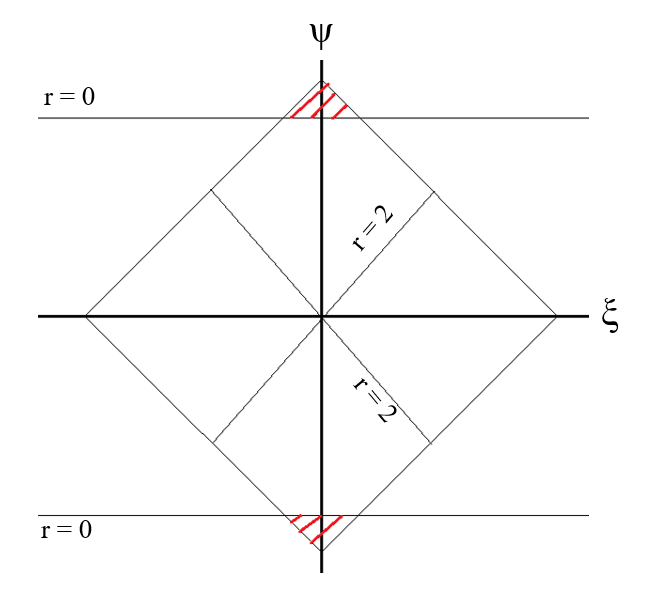
\includegraphics[width=0.9\linewidth]{img/carter-penrose2}
	\end{minipage}
	\caption{Plots of lines of constant r and t when looking at the relation between U,T (left). The same image conformally shifted to new variables (right).}
	\label{fig:Figure6.1}
	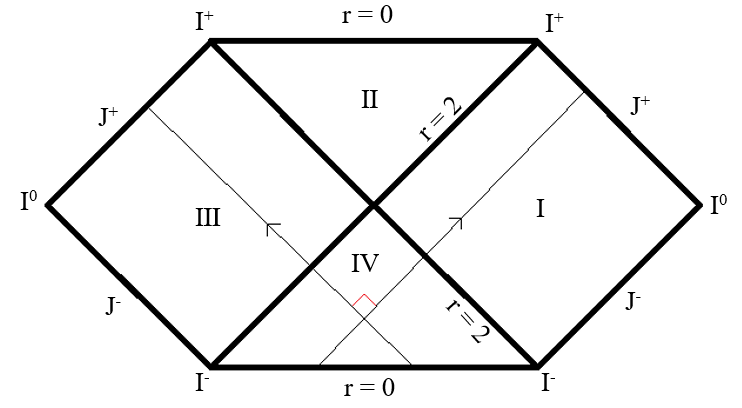
\includegraphics[width=0.6\linewidth]{img/carter-penrose3}
	\caption{A common representation of a Carter-Penrose diagram of the maximal analytic extension of the Schwarzschild metric.}
	\label{fig:Figure6.2}
\end{figure}

\vspace{1em}
	In figure \ref{fig:Figure6.2}, region \RomanNumeralCaps{1} is the outside of the black hole in our universe, region \RomanNumeralCaps{2} is the outside of the black hole in some other universe, region \RomanNumeralCaps{3} is the inside of the black hole in our universe, and region \RomanNumeralCaps{4} is the inside of some 'white hole'. In this Carter-Penrose diagram, null geodesics are represented by straight lines (moving upwards) at a 45 degree angle; from this we see that any worldline from a point in region \RomanNumeralCaps{2} ends at the singularity r=0, this fits our description of the inside of a black hole.

\vspace{1em}
	We name region \RomanNumeralCaps{4} a white hole as it holds the opposite properties; any wordline which finds itself inside region \RomanNumeralCaps{4} inevitably escapes into regions \RomanNumeralCaps{1} and \RomanNumeralCaps{2}. Also note no geodesics may enter region \RomanNumeralCaps{4}, and no geodesics may cross from region \RomanNumeralCaps{1} to region \RomanNumeralCaps{2}. This stands to reason as the Schwarzschild metric cannot be used to model a wormhole, since any geodesic crossing the event horizon will intersect the singularity (notably unlike the Kerr metric).

\subsection{Extending the Kerr metric}\label{subsec:Section6.1.2}

	Using the methods discussed for the Schwarzschild metric above, one can derive a maximal analytic extension of the Kerr metric, as was done by Boyer and Lindquist. The purpose of the above subsection was to give readers a flavour of what such a derivation looks like, without having to go through the more arduous task of doing so for the Kerr metric. 

\vspace{1em}
	Beyond this point in the chapter, we must give full credit to Alaine Riazuelo, as all figures and content are either his from his paper Seeing Relativity \RomanNumeralCaps{3}\cite{seeingRelativity}, or a rewording and restructuring of his paper to give readers a sense of the current cutting edge of the field of relativistic modelling.

\vspace{1em}
	We will use an extension taken by Riazuelo, and may construct a Carter-Penrose diagram for this extension to use in analysis of images formed at various points along a plunging path through the ring singularity. A Carter-Penrose diagram gives us the causal structure of a metric and its regions, allowing us to clearly see which geodesics may reach an observer at a given point if we know what allowed paths for geodesics in the diagram are, for this reason one of our first tasks will be to list possible geodesic paths.

\vspace{1em}
\begin{figure}[!ht]
	\centering
	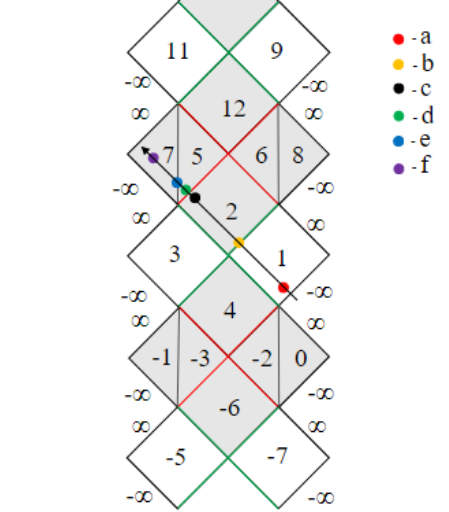
\includegraphics[width=0.5\linewidth]{img/carter-penrose-kerr}
	\caption{A Carter-Penrose diagram of the maximal analytic extension of the Kerr metric.}
	\label{fig:Figure6.3}
\end{figure}

\vspace{1em}
	In figure \ref{fig:Figure6.3}, region 1 is our universe, regions 0 and 8 are the Kerr black hole, and regions -7, -5, 3 and 9 are the 'other universe'. The boundaries coloured green are the outer horizon of the black hole, and the boundaries coloured in red are the inner horizon. The boundary between regions 5 and 7 is the ring singularity. The plunging trajectory we take is shown as an arrow on the diagram, with various points along the trajectory picked out; these are points for which Riazuelo generated images. The full Carter-Penrose diagram is an infinite extension of this diagram but enough blocks are shown here to cover all regions.

\vspace{1em}
	The celestial sphere used for region 1 is the starless Milky Way taken by the Two-Micron All-Sky Survey\cite{skrutskie2006two}. Region 3; a kind of 'twin' to region 1, has a high-frequency dominated image of the Milky Way taken by the Planck satellite after a one-year full-sky survey\cite{planck2011astronomy}.

\vspace{1em}
	Regions 7 and -1 take cosmic background microwave radiation maps from the Planck satellite\cite{adam2016planck}. Similarly, region 8 shows a temperature map generated by the Wilkinson Microwave Anisotropy Probe\cite{bennet2013wmap}. Note that regions 7 and -1 are not seen at the same time nor in quick succession, so there may be no confusion as to which region is being shown given the Carter-Penrose diagram.

\vspace{1em}
	Finally region -7 is a generated map of greyscale patches with orange polar regions. Different colours were applied for equatorial bands (northern band = very light grey, southern band = very dark grey), also distinguishing colours were used for 4 meridians situated 90 degrees apart from one another (red, black, light grey and white).

\section{Falling into a Kerr black hole}\label{sec:Section6.2}

\vspace{1em}
	Here we shall discuss the alllowed paths of null geodesics to be able to analyse generated images, any example paths which I give here are applicable if they are equivalent modulo 8:

\vspace{1em}
\begin{itemize}
  \item Geodesics which never leave their region: For some regions such as region 1, there are geodesics which may originate and stay inside of one region.
  \item Returning geodesics (two kinds): Two kinds of geodesics starting at r=$\infty$ which cross the inner and outer horizons, then return to some asymptotic regions, an example of such a path is 1, 2, 5, 12, 9. The second type has its turning point inside of the negative r region 1, 2, 5, 7, 5, 12, 9.
  \item Ingoing transit geodesics: Geodesics starting at r=$\infty$ and ending at r=-$\infty$ and their mirror partner e.g. 1, 2, 5, 7 and 3, 2, 6, 8.
  \item Outgoing transit geodesics: Geodesics starting at r=-$\infty$ and ending at r=$\infty$ and their mirror.
  \item Bounded geodesics: There are four infinite sequences so-called bounded geodesics may take, as implied by the infinite nature they are self-repeating, The four sequences being (1, 2, 5, 12, 9). (1, 2, 6, 12, 9). (3, 2, 5, 12, 11). (3, 2, 6, 12, 11). Note that the first kind of returning geodesic is a bounded geodesic.
\end{itemize}

\vspace{1em}
	In the first image of figure \ref{fig:Figure6.4}, taken at r=6M, we see mostly our universe, with some of region -7 shown due to bounded geodesic paths. The second image, taken at r=1.6781M, is a distorted image of the gravitational lensing of a Kerr black hole, with a very small image of region -7 this is as there are fewer bounded geodesics closer to the boundary to region 2 due to the nature of the path taken. 

\vspace{1em}
\begin{figure}[!ht]
	\centering
	\begin{minipage}{0.5\textwidth}
		\centering
		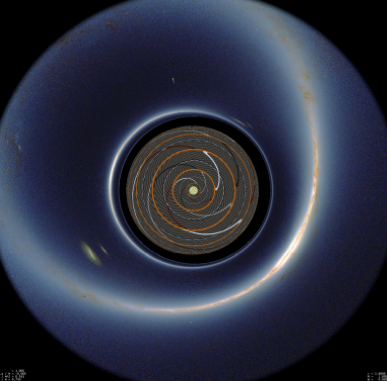
\includegraphics[width=0.75\linewidth]{img/plunging1}
	\end{minipage}%
	\hfill
	\begin{minipage}{0.5\textwidth}
		\centering
		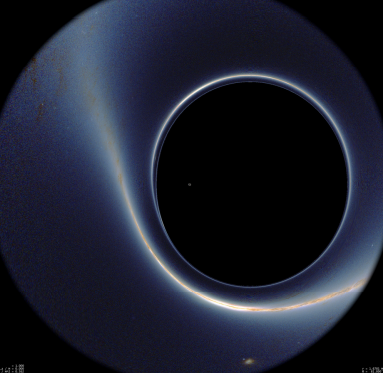
\includegraphics[width=0.75\linewidth]{img/plunging2}
	\end{minipage}
	\caption{Points a (r=6M) (left), and b (r=1.6781M) (right).}
	\label{fig:Figure6.4}
\end{figure}

\vspace{1em}
	In the image generated at point c (see figure \ref{fig:Figure6.5} (left)), taken at r=0.3389M, we still see our universe due to our past light cone, though heavily distorted now. We also see a large amount of region 3, this is because there are both outgoing transit geodesics and two kinds of bounded geodesics moving from region 3 into region 2 leading to three possible kinds of paths light may take from region 3 into region 2.

\vspace{1em}
\begin{figure}[!ht]
	\centering
	\begin{minipage}{0.5\textwidth}
		\centering
		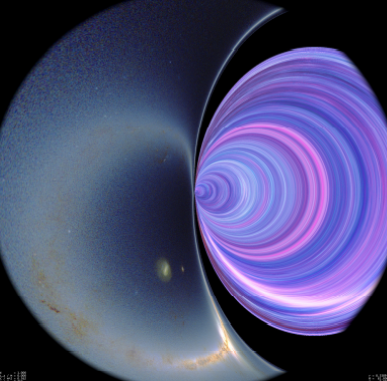
\includegraphics[width=0.75\linewidth]{img/plunging3}
	\end{minipage}%
	\hfill
	\begin{minipage}{0.5\textwidth}
		\centering
		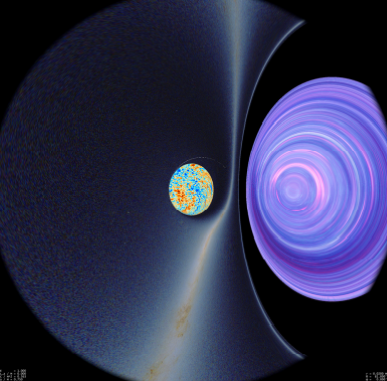
\includegraphics[width=0.75\linewidth]{img/plunging4}
	\end{minipage}
	\caption{Points c (r=0.3389M) (left), and d (r=0.012M) (right).}
	\label{fig:Figure6.5}
\end{figure}

\vspace{1em}
	In the next image, modelling an observer at point d, taken at r=0.012M, we still see regions 1 (our universe) and 3, but we now observe energy from region 7 due to outgoing transit geodesics and bounded geodesics. We can now see the highlighted ring singularity of the Kerr black hole, though very finely. The reason we see light rays from region 1 inside the ring singularity is due to the second kind of returning geodesic, which Riazuelo dubs adventurous geodesics, entering and quickly exiting the negative r region.

\vspace{1em}
	Perhaps unsurprisingly crossing the ring singularity makes no real change save the lack of highlighted ring singularity itself, this is because the crossing is mundane, that is to say it is not a sudden crossing such that no past light rays may reach you, there are still plenty of past light rays which follow a null geodesic to reach the same point as you.

\vspace{1em}
	However, distortion exponentially increases in region 7 so a small shift in position significantly affects the amount of past light rays observed and the amount of distortion. We see this in the images generated at the points e$_1$ and e$_2$ (see figure \ref{fig:Figure6.6}), which are points just before and after crossing the ring singularity. Since there are no bounded geodesics which can touch the ring singularity, there are no reasonable bounded geodesics at e$_1$ from region 3, meaning we no longer see its purple hue.

\vspace{1em}
\begin{figure}[!ht]
	\centering
	\begin{minipage}{0.5\textwidth}
		\centering
		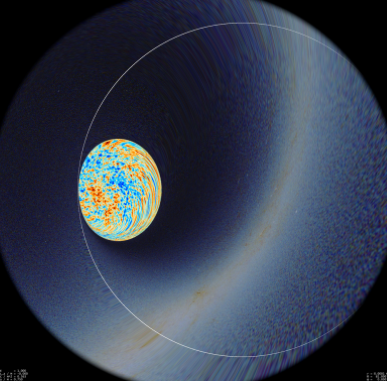
\includegraphics[width=0.75\linewidth]{img/plunging5-1}
	\end{minipage}%
	\hfill
	\begin{minipage}{0.5\textwidth}
		\centering
		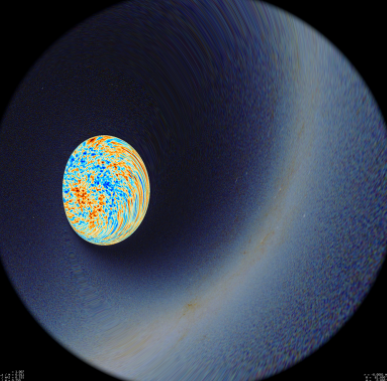
\includegraphics[width=0.75\linewidth]{img/plunging5-2}
	\end{minipage}
	\caption{Points e$_1$ (r=0.0001M) (left), and e$_2$ (r=-0.0001M) (right).}
	\label{fig:Figure6.6}
\end{figure}

\vspace{1em}
	Finally, in figure \ref{fig:Figure6.6}, we see an image of what an observer would see at r=-0.512M, with only a small 'connection' back to where it started in our universe. Interestingly this image looks like a distorted kind of inverse version of our image taken at point a, almost all geodesics observed are geodesics which are contained in their region, which can only be said for the first and final images, giving a sense of circularity and closure.

\begin{figure}[!ht]
	\centering
	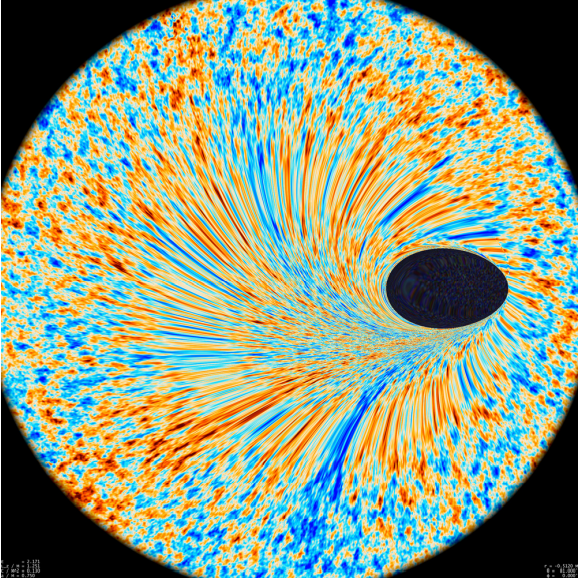
\includegraphics[width=0.6\linewidth]{img/plunging6}
	\caption{Point f: r=-0.512M.}
	\label{fig:Figure6.7}
\end{figure}


\begin{conclusion}
	We have now covered a large amount of some of the core ideas and developments in the field of relativistic modelling. Of course, there are many topic-adjacent areas which we have not been able to touch on or expand upon, but to avoid this paper becoming unreasonably long, it is here we shall finish. 

\vspace{1em}
	We have moved from the Prussian Academy of Sciences in 1915, with Albert Einstein introducing a revolutionary concept, all the way through to recently published papers on, or close to, the cutting edge of the field with regard to physical implications. It is my hope that readers will come away with some new knowledge from this paper regardless of academic background; whether that be the origins and use of general relativity, or what a model of an observer in a maximal analytic extension of the Kerr metric may see.

\vspace{1em}
	Just to name a few of the areas in which our focus has not landed upon; readers may want to move on from this paper by exploring papers by Mandal\cite{mandal2021non}, Pu\cite{pu2016odyssey} and Thomas Muller\cite{muller2021adaptive} on alternate methods with a focus on the improvement of computational efficiency - a particularly important goal with blockbuster films requiring minutes of IMAX quality renders. As discussed in section \ref{sec:Section5.1} there are many papers on physical models of accretion discs, to varying degrees of accuracy at the cost of complexity. Relativistic raytracing has been used on various other key metrics, including the Kerr-Newman metric, which best describes naturally occurring black holes in our universe, and Ellis-Thorne wormholes\cite{thorne2015visualizing}.

\vspace{1em}
	 The field of general relativity, even when narrowed down to black holes, is incredibly informative to the way in which our universe functions. The study of black holes has advanced the scientific community for over 100 years, and will likely continue to do so.
\end{conclusion}


\appendix
\chapter{Final Code}
\begin{lstlisting}
from numpy import pi, sin, cos, sqrt, arctan, arccos
from scipy.integrate import solve_ivp
import matplotlib.pyplot as plt
from PIL import Image

img=Image.open("C:/Users/user/example.png")
imageCopy=Image.open("C:/Users/user/example.png")
accretionimage=Image.open("C:/Users/user/example-accretion.png")

width=img.size[0]
height=img.size[1]
halfWidth=int(width/2)
halfHeight=int(height/2)
celestialr = 100


#Initial conditions
r, theta, phi = [74.1, 1.511, 0]
v = 1
a = -0.999
x0 = sqrt(r**2+a**2)*sin(theta)*cos(phi)
y0 = sqrt(r**2+a**2)*sin(theta)*sin(phi)
z0 = r*cos(theta)
counter1=0
counter2=0


#Run over each pixel
for j in range(height):
    for i in range(width):
        counter1+=1
        if counter1%int(height*width/100)==0:
            counter2+=1
            counter1=0
            print(counter2)
            
            
        #Convert to familiar coordinates with centre pixel being (0,0)
        pixx=i-halfWidth
        pixy=halfHeight-j
        
        #Convert to angles
        x=pixx*pi/height
        y=pixy*pi/height
        
        #Find final position (Cartesian)
        xend=x0+celestialr*sin(x)*cos(y)
        yend=y0+celestialr*sin(y)
        zend=z0+celestialr*cos(x)*cos(y)
        endlen = sqrt((xend-x0)**2+(yend-y0)**2)
        
        
        #Find launch and inclination angles
        if zend == z0:
            launch = 3*pi/2+pi/2
        else:
            launch = 3*pi/2+arccos((zend-z0)/celestialr)  
        if x==0:
            if y>0:
                incl=pi
            else:
                incl=pi+pi
        elif endlen == 0:
            incl=0
        elif y>=0:
            incl = pi/2+arccos((xend-x0)/endlen)
        else:
            incl = pi/2-arccos((xend-x0)/endlen)
        
        #More initial conditions
        vr = v*sin(launch)
        vphi = v*cos(launch)*sin(incl)
        vtheta = v*cos(launch)*cos(incl)
        
        #Define useful functions
        def Sigma(r, theta):
            return (a*cos(theta))**2 + r**2
        def Delta(r):
            return a**2 + r**2 - 2*r
        def Chi(r, theta):
            return (r**2 + a**2)**2 - Delta(r)*(a*sin(theta))**2

        L = vphi*sin(theta)*sqrt(Chi(r, theta)/Sigma(r, theta))
        omega = 2*r*a/Chi(r, theta)
        E = sqrt(Delta(r)*Sigma(r, theta)/Chi(r, theta)) + L*omega
        ptheta = vtheta*sqrt(Sigma(r, theta))
        pr = vr*sqrt((Sigma(r, theta)/Delta(r)))
        Q = ptheta**2 + ((L/sin(theta))**2 - (a*E)**2)*(cos(theta)**2)
        k = Q + L**2 + a**2*E**2
        
        #Initial condition list
        varlist = [0, r, theta, phi, pr, ptheta]
        
        
        # ODE solver parameters
        eh = 1 + (1 - a**2)**(1/2)
        def event(tau, X):
            return abs(X[1]) - eh
        event.terminal=True
        
        #Comment out if no accretion disc
        inneraccretionr=9.61
        accretionr=18.7
        proportionacc=(accretionimage.size[0]-1)/(2*accretionr)
        def event1(tau, X):
            return 500*abs(cos(X[2])) + abs(X[1])**2-(inneraccretionr+accretionr)*abs(X[1])+inneraccretionr*accretionr
        event1.terminal=True
        
        #ODE system
        def mydiff(tau, X=varlist):
            t, r, theta, phi, pr, ptheta = X
            td = E + (2*r*(r**2 + a**2)*E - 2*a*r*L)/(Sigma(r, theta)*Delta(r))
            rd = pr*Delta(r)/Sigma(r, theta)
            thetad = ptheta/Sigma(r, theta)
            phid = (2*a*r*E + (Sigma(r, theta) - 2*r)*L/(sin(theta)**2))/(Sigma(r, theta)*Delta(r))
            prd = 1/(Sigma(r, theta)*Delta(r))*(-k*(r - 1)+2*r*(r**2 + a**2)*E**2 - 2*a*E*L) - (2*pr**2*(r - 1))/Sigma(r, theta)
            pthetad = (sin(theta)*cos(theta))/(Sigma(r, theta))*(L**2/(sin(theta)**4) - (a*E)**2)
            return [td, rd, thetad, phid, prd, pthetad]           
        
        #Solve
        sol = solve_ivp(mydiff, [-celestialr,0], varlist, events=[event,event1])

        rlst = sol.y[1]
        thetalst=sol.y[2]
        philst=sol.y[3]
        
        #Update final pixel
        if len(sol.y_events[0])>0 or abs(rlst[-1])<=5:
            #Entered EH/Trapped in ergosphere
            img.putpixel((i,j),(0,0,0))
        elif len(sol.y_events[1])>0:
            #Hit accretion disc
            finalaccpixx=(rlst[-1]*proportionacc*cos(philst[-1])+accretionimage.size[0]/2)%accretionimage.size[0]
            finalaccpixy=(rlst[-1]*proportionacc*sin(philst[-1])-accretionimage.size[1]/2)%accretionimage.size[0]
            img.putpixel((i,j),accretionimage.getpixel((finalaccpixx,finalaccpixy)))
        else:
            #Compute final position (Cartesian)
            x1 = sqrt(rlst[-1]**2+a**2)*sin(thetalst[-1])*cos(philst[-1])
            y1 = sqrt(rlst[-1]**2+a**2)*sin(thetalst[-1])*sin(philst[-1])
            z1 = rlst[-1]*cos(thetalst[-1])
            #Compute angles to final position
            if y1>y0:
                endtheta = arctan((x1-x0)/(y1-y0))
                endphi = -arctan((z1-z0)/(sqrt((x1-x0)**2+(y1-y0)**2)))
            elif y1<y0:
                endtheta = pi + arctan((x1-x0)/(y1-y0))
                endphi = -arctan((z1-z0)/(sqrt((x1-x0)**2+(y1-y0)**2)))
            
            #Convert angles to pixels
            endpixx = int(height+halfHeight+int(endtheta*height/pi))%width
            endpixy = (halfHeight+int(endphi*height/pi))%height

            img.putpixel((i,j),imageCopy.getpixel((endpixx,endpixy)))
            
#Show and save image
figure, ax = plt.subplots()
ax.axis("equal")
ax.get_xaxis().set_visible(False)
ax.get_yaxis().set_visible(False)
img.save("C:/Users/user/example-final-product.png")        

plt.imshow(img)
plt.show()
\end{lstlisting}





%\nocite{}
%\bibliographystyle{ieeetr}
\bibliographystyle{unsrt}
\bibliography{bibliography}{}
\end{document}